\documentclass[11pt,twoside,a4paper]{book}  
% definice dokumentu
\usepackage[czech, english]{babel}
\usepackage[T1]{fontenc} 				% pouzije EC fonty 
\usepackage[utf8]{inputenc} 			% utf8 kódování vstupu 
\usepackage[square, numbers]{natbib}	% sazba pouzite literatury
\usepackage{indentfirst} 				% 1. odstavec jako v cestine, pro práci v aj možno zakomentovat
\usepackage{fancyhdr}					% tisk hlaviček a patiček stránek
\usepackage{nomencl} 					% umožňuje snadno definovat zkratky a jejich seznam

%%%%%%%%%%%%%%%%%%%%%%%%%%%%%%%%%%%%%%%%%%%%%%%%%%%%%%%%%%%%%%%
% informace o práci
\newcommand\WorkTitle{Analýza a návrh abstraktní vícevrstvé architektury pro práci s grafovou databází realizující metadatové úložiště pro data lineage}
\newcommand\FirstandFamilyName{Bc. Jakub Moravec}															
\newcommand\Supervisor{Ing. Michal Valenta, Ph.D.}															

\newcommand\TypeOfWork{Diplomová práce}	

\newcommand\StudProgram{Otevřená Informatika, Magisterský}	% program
\newcommand\StudBranch{Softwarové inženýrství}				% obor

%%%%%%%%%%%%%%%%%%%%%%%%%%%%%%%%%%%%%%%%%%%%%%%%%%%%%%%%%%%%%%%
% minimální importy
\usepackage{graphicx}					% pro vkládání obrázků
\usepackage{k336_thesis_macros} 		% specialni makra pro formatovani DP a BP
\usepackage[
pdftitle={\WorkTitle},				% nastaví v informacích o pdf název
pdfauthor={\FirstandFamilyName},	% nastaví v informacích o pdf autora
colorlinks=true,					% před tiskem doporučujeme nastavit na false, aby odkazy a url nebyly šedé při ČB tisku
breaklinks=true,
urlcolor=red,
citecolor=blue,
linkcolor=blue,
unicode=true,
]
{hyperref}								% pro zobrazování "prokliknutelných" linků 

% rozšiřující importy
\usepackage{listings} 			%slouží pro tisk zdrojových kódů se syntax higlighting
\usepackage{algorithmicx} 		%slouží pro zápis algoritmů
\usepackage{algpseudocode} 		%slouží pro výpis pseudokódu
\usepackage{amsmath}            %vzorce
\usepackage[dvipsnames]{xcolor} % barvy

%%%%%%%%%%%%%%%%%%%%%%%%%%%%%%%%%%%%%%%%%%%%%%%%%%%%%%%%%%%%%%%
% příkazy šablony
\makenomenclature								% při překladu zajistí vytvoření pracovního souboru se seznamem zkratek

\let\oldUrl\url									% url adresy budou zobrazeny: <url> 
\renewcommand\url[1]{<\texttt{\oldUrl{#1}}>}

%%%%%%%%%%%%%%%%%%%%%%%%%%%%%%%%%%%%%%%%%%%%%%%%%%%%%%%%%%%%%%%
% vaše vlastní příkazy
\newcommand*{\nomExpl}[2]{#2 (#1)\nomenclature{#1}{#2}} 	% usnadňuje zápis zkratek : Slova ke Zkrácení (SZ)
\newcommand*{\nom}[2]{#1\nomenclature{#1}{#2}} 			% usnadňuje zápis zkratek : SZ

%%%%%%%%%%%%%%%%%%%%%%%%%%%%%%%%%%%%%%%%%%%%%%%%%%%%%%%%%%%%%%%
% listings syntax highlighting

\renewcommand{\lstlistingname}{Příklad}% Listing -> Příklad
\renewcommand{\lstlistlistingname}{Seznam příkladů}% List of Listings -> List of Algorithms

\lstset{ %
  backgroundcolor=\color{white},   % choose the background color
  basicstyle=\footnotesize,        % size of fonts used for the code
  breaklines=true,                 % automatic line breaking only at whitespace
  captionpos=b,                    % sets the caption-position to bottom
  commentstyle=\color{OliveGreen},    % comment style
  escapeinside={\%*}{*)},          % if you want to add LaTeX within your code
  keywordstyle=\color{blue},       % keyword style
  stringstyle=\color{red},     % string literal style
}


%%%%%%%%%%%%%%%%%%%%%%%%%%%%%%%%%%%%%%%%%%%%%%%%%%%%%%%%%%%%%%%
% vlastní dokument
%%%%%%%%%%%%%%%%%%%%%%%%%%%%%%%%%%%%%%%%%%%%%%%%%%%%%%%%%%%%%%%
\begin{document}
	
	%%%%%%%%%%%%%%%%%%%%%%%%%% 
	% nastavení jazyka, kterým je práce psána
	\selectlanguage{czech}	% podle jazyka práce nastavte na [czech | english]
	\translate				% nastaví české nebo anglické popisy (např. katedra -> department); viz k336_thesis_macros

	%%%%%%%%%%%%%%%%%%%%%%%%%%    
	% Poznamky ke kompletaci prace
	% Nasledujici pasaz uzavrenou v {} ve sve praci samozrejme 
	% zakomentujte nebo odstrante. 
	% Ve vysledne svazane praci bude nahrazena skutecnym 
	% oficialnim zadanim vasi prace.
	{
	\pagenumbering{roman} \cleardoublepage \thispagestyle{empty}
	\chapter*{Na tomto místě bude oficiální zadání vaší práce}
	\begin{itemize}
		\item Toto zadání je podepsané děkanem a vedoucím katedry,
		\item musíte si ho vyzvednout na studijním oddělení Katedry počítačů na Karlově náměstí,
		\item v jedné odevzdané práci bude originál tohoto zadání (originál zůstává po obhajobě na katedře),
		\item ve druhé bude na stejném místě neověřená kopie tohoto dokumentu (tato se vám vrátí po obhajobě).
	\end{itemize}
	\newpage
	}

	%%%%%%%%%%%%%%%%%%%%%%%%%%    
	% Titulni stranka / Title page 
	\coverpagestarts

	%%%%%%%%%%%%%%%%%%%%%%%%%%%    
	% Poděkovani / Acknowledgements 

	\acknowledgements
	\noindent
	Zde můžete napsat své poděkování, pokud chcete a máte komu děkovat.


	%%%%%%%%%%%%%%%%%%%%%%%%%%%   
	% Prohlášení / Declaration 

	\declaration{V~Kořenovicích nad Bečvárkou dne 15.\,5.\,2008}
	%\declaration{In Kořenovice nad Bečvárkou on May 15, 2008}


	%%%%%%%%%%%%%%%%%%%%%%%%%%%%    
	% Abstrakt / Abstract 
 
	\abstractpage

	Translation of Czech abstract into English.

	\vglue60mm

	\noindent{\Huge \textbf{Abstrakt}}
	\vskip 2.75\baselineskip

	\noindent
	Abstrakt práce by měl velmi stručně vystihovat její obsah. Tedy čím se práce zabývá a co je jejím výsledkem/přínosem.

	\noindent
	Očekávají se cca 1 -- 2 odstavce, maximálně půl stránky.

	%%%%%%%%%%%%%%%%%%%%%%%%%%    
	% obsahy a seznamy
	\tableofcontents		% Obsah / Table of Contents 

	% pokud v práci nejsou obrázky nebo tabulky - odstraňte jejich seznam
	\listoffigures			% Obsah / Table of Contents 
	\listoftables			% Seznam tabulek / List of Tables
	\lstlistoflistings         % Seznam kódů

	%%%%%%%%%%%%%%%%%%%%%%%%%% 
	% začátek textu  
	\mainbodystarts

\chapter{Úvod}
\label{sec:uvod}
\section{Data lineage}

% Úvod
Data a z nich získávané informace vždy byly v centru pozornosti informačních technologií a jejich význam každým rokem stoupá. V digitální podobě jsou dnes zakódovány takřka všechny informace včetně našich osobních údajů, bankonvních transakcí, či zdravotních informací. Zároveň stále roste roste množství těchto dat\footnote{Podle statistiky IDC \cite{Idc14} se celkový objem dat virtuálního světa zdvojnásobuje každé dva roky.}.
Je tedy kladena velká pozornost na procesy, kterými jsou data zpracovávána a pomocí kterých jsou z dat získávány informace. Existuje několik přístupů k tomuto problému, ať už se jedná o tradiční relační databázové systémy, datové sklady a \textit{\nomExpl{OLAP}{Online Analytical Processing}} analytické nástroje, \textit{data miningové} technologie, nebo novější obory, jako jsou \textit{NoSQL} databáze a analytické nástroje. Ať už je zvolen kterýkoliv z těchto přístupů, procesy zpracovávající data bývají komplexní a často ne zcela intuitivní pro samotné vývojáři, natož potom pro analytiky či dokonce byznys uživatele.

% Data Lineage
Do popředí se tak dostává nová skupina nástrojů označovaných jako Data lineage.\footnote{Stejně jako mnoho další termínů z oblasti informačních technologií se Data lineage nepřekládá, nebudeme ho tedy překládat ani my. Pokud bychom termín však přeci jen chtěli popsat českými slovy, nejvhodnější překlad by byl zřejmě "řízení datových toků".}
Jejich cílem je analyzovat end-to-end datové toky v systému - zdroje, transformace a cíle dat a pomocí této analýzy umožnit uživateli vhled do tohoto procesu. To může být velmi komplexní úkol, informační systém se typicky skládá z řady navzájem propojených technologií, a nástroj pro analýzu Data lineage si musí umět poradit nejen s každým z nich separátně, ale také s případnými transformacemi na hranicích těchto systémů.

% Manta Flow
Jedním z úspěšných nástrojů pro Data lineage je \textit{Manta Flow}\footnote{\url{https://getmanta.com/}}. Nástroj analyzuje zdrojové kódy vybraných RDBMS databází, Big Data nástrojů a ETL nástrojů.
Zdrojové kódy analyzovaných systémů jsou pravidelně parsovány dle syntaktických a sémantických pravidel podporovaných nástrojů a následně jsou analyzovány přímé a nepřímé\footnote{Představme si relační databázi s tabulkami \textit{A}, \textit{B} a \textit{C}. Představme si, že data z tabulky \textit{A} jsou \textit{ETL transformací} přenesena do tabulku \textit{B}. Tato \textit{ETL transformace} filtruje data z tabulky \textit{A} dle dat z tabulky \textit{C}. Potom z tabulky \textit{A} do tabulky \textit{B} vede \textit{přímý datový tok} a z tabulky \textit{C} do tabulky \textit{B} vede \textit{nepřímý datový tok}.} datové toky a transformace dat v informačním systému.
Získané informace jsou ukládány do metadatového uložiště, jímž je v současné době grafová databáze \textit{Titan}\footnote{\url{http://titan.thinkaurelius.com/}}. Klientská část aplikace potom umožňuje uživateli vizualizovat datové toky dle zadaných parametrů (zdroj a cíl datového toku, úroveň abstrakce atd.). Dynamicky tak vznikají komplexní dotazy do metadatové databáze, pomocí kterých jsou procházeny grafy datových toků a vraceny výsledky.

\section{Definice problému}
% Neexistence standardů GDB
Přestože má použití grafové databáze jako metadatového uložiště pro Data lineage nástroje silné opodstatnění\footnote{Grafová databáze umožňuje výrazně rychlejší hledání datových toků v informačních systémech, než by umožňovali jiné architektury. Způsob procházení grafů je popsán v kapitole \ref{sec:gdb-dotazy}.}, přináší s sebou krom nesporných výhod také řadu problémů. Jejich společným jmenovatelem je fakt, že v oblasti grafových databází, která je relativně nová a stále prochází dynamickým rozvojem, nejsou zatím jasně definovány obecně podporované standardy. Neexistuje například univerzální, stabilní a obecně podporovaný dotazovací jazyk pro grafové databáze (například v oblasti relačních databází tuto úlohu plní SQL). To vede mimo jiné k tomu, že nejsou v tuto chvíli definovány doporučené postupy softwarového inženýrství pro tvorbu abstraktních rozhraní pracujících s grafovými databázemi. Není tak překvapaním, že je při používání grafových databází v aplikacích často míchána perzistentní a byznys logika aplikace, což je typickou ukázkou špatného návrhu\cite{Taylor09}. Pro produkt \textit{Manta Flow} je tento problém velice aktuální - používaná databáze \textit{Titan} již není dále vyvýjena, brzy skončí její podpora \cite{Titan04} a je pravděpodobné, že dojde k její výměně za jinou technologii. Cílem této práce je navrhnout abstraktní architekturu pro práci s grafovou databází, která bude vyhovovat potřebám nástroje \textit{Manta Flow} a bude v co největší míře oddělovat perzistentní logiku od zbytku aplikace. Zavedení této vrstvy aplikace bude pravděpodobně znamenat zásah do celé architektury aplikace. Součástí práce tedy musí být nový návrh architektury aplikace reflektující změnu v přístupu ke grafové databází.

\section{Struktura diplomové práce}
Práce je rozdělena na teoretickou a experimentální část.

% Teorietická část
Cílem teoretické části je popsat obecné principy grafových databází, jejich vnitřní organizaci a možnosti dotazování dat. Dále jsou popsány možnosti abstrakce ve světě softwarového inženýrství - ať už na úrovní procesů a programových rozhraní (API), nebo na nižších úrovních - například návrhových vzorů.

%Experimentální část
Experimentální část práce obsahuje hlubší analýzu potřeb projektu \textit{Manta Flow} pro přístup ke grafové databázi. Na základě teoretické části práce je navržena vícevrstvá abstraktní architektura, vytvořeno \nomExpl{PoC}{Proof of Concept} řešní a to otestováno nad reálnými data.

\chapter{Teoretická část}

%%%%%%%%%%%%%%%%%%%%%%%%%%%%%%%%%%%%%%%%%%%%%%%%%
\section{Grafové databáze}
\label{sec:gdb}

Grafy jsou velice přirozeným způsobem reprezentaci dat, zvláště v době, kdy většina dat je vytvářena uživateli a není strukturovaná. Grafy pomocí uzlů a hran přirozeně popisují objekty a vztahy mezi nimi, nevynucují náročné datové modelování skutečnosti do složitých datových struktur a usnadňují tak proces objevování informací v datech. Díky tomu, že grafy umožňují jednoduché prohledávání objektů, které mezi sebou mají vztahy (uzlů propojených hranami), jsou operace tohoto typu nad grafy relativně (například vůči relačním databázím) rychlé.

Grafové databáze umožňují data reprezentovaná grafem ukládat a procházet tak, aby byly tyto přirozené výhody grafů zachovány a v některých případech byly také zajištěny některé vlastnosti relačních databázových systémů (jako například atomicitu transakcí). Problémů, pro které je vhodné využití grafových databází je mnoho, příkladem může být ochrana proti podvodům v bankovním sektoru. Některé vzorce v datech je složité odhalit pomocí modelů relačních databází. Grafové databáze naopak přináší nový pohled na data a implicitně ukazují vztahy mezi nimi. Umožňují tak odhalit v datech více podezřelých vzorců, které často mohou znamen právě bankovní podvody.\cite{Webber17} Dalším z mnoha příkladů jsou také řešení v oblasti \textit{data lineage}, která si kladou za cíl sledovat vztahy mezi daty společností a mapovat proces jejich zpracování.

Tato kapitola má za cíl představit základní principy grafových databází. Popisuje reprezentaci grafů v databázi, možnosti analýzy dat a rozhraní, kterých je k tomu možné použít.

\subsection{NoSQL databáze}
\label{sec:gdb-nosql}
NoSQL databázové sice nejsou předmětem této práce, grafové databáze nicméně bývají zařazovány jako podkategorie NoSQL a proto zde základní principy této skupiny technologií popíšeme. Samotná zkratka NoSQL je vykládaná různě, většinou jako \textit{"Not only SQL"} \cite{Evans09} a vykládá se jako označení pro databáze nerelačního typu určené pro zpracování \textit{Big Data}\footnote{Big Data jsou soubory dat velkého objemu, velké rychlosti a/nebo velké různorodosti, která vyžadují nové formy zpracování pro umožnění lepšího rozhodování, většího porozumění domény a optimalizace procesů.\cite{Laney01}}. Mezi hlavní uváděné výhody NoSQL databází patří:

\begin{itemize}
  \item{\textit{Škálovatelnost:}} Zatímco klasické databázové systémy využívají \textit{vertikální škálovatelnost}, NoSQL databáze umožňují efektivní \textit{horizntální škálování}. \textit{Vertikální škálování} je prováděno pomocí navýšení zdrojů (ať už výpočetní kapacity, nebo paměti) jednoho zařízení, což má své technické a ekonomické limity. Na druhé straně u horizontálně škálovatelného systému, lze navýšit jeho výkon a/nebo kapacitu přidáním dalšího zařízení. Jedná se tedy o síť spolupracujících zařízení. Data v NoSQL databázích bývají typicky distribuovaná na několik uzlů\footnote{Pojem cluster může mít několik významů, zde je požíván jako množina síťově propojených počítačů.} a jejich zpracování tak může probíhat paralelně.
  \item{\textit{Efektivní čtení:}} NoSQL datatabáze jsou silně orientovány na rychlé čtení (koncept \textit{write once, read many times}). Ve většině již nejsou data po zapsání do databáze nikdy modifikována, pouze nad nimi jsou vykonávány analýzy (dotazy). Za cenu potenciálně pomalejšího zápisu dat do databáze (který nám nevadí) získáme tedy výrazně vyšší rychlost čtení dat.
  \item{\textit{Flexibilní datový model:}} NoSQL databáze buď nevyžadují žádné datové schéma, nebo je schéma volné (a lze ho tedy upravovat bez nutnosti úpravy stávajících dat). Dodržování schématu dat je tedy na aplikaci, která NoSQL databázi používá.
  \item{\textit{Ekonomická stránka:}} jak již bylo uvedeno, relační databáze je nutné typicky škálovat vertikálně a to je nákladné - jsou navyšovány prostředky jednoho stroje (serveru), což má technická omezení a čím více se těmto omezením blížíme, tím je škálování dražší. Vedlejším efektem této skutečnosti je často také \textit{vendor-locking}, tedy situace, kdy jsme nuceni používat specifický hardware (často od jedné konkrétní společnosti), který je velmi nákladný. Na druhé horizontální škálování je relativně levné - škáluje se přidáním nového uzlu. Vzhledem k tomu, že NoSQL databáze nevyžadují specifický hardware, je možné používat takzvaný \textit{komoditní hardware} (uzly nemusí být hardwarově homogenní), který je levný.
\end{itemize}

Aby těchto výhod NoSQL databáze dosáhly, využívají různé přístupy k reprezentaci dat a manipulaci s daty. Jejich hlavní rozdělení je následující:

% Typy NoSQL databází
\begin{itemize}
  \item{\textit{Databáze typu klíč-hodnota:}} Tyto databáze mají zcela volné datové schéma, jsou realizovány jako mapa klíčů a hodnot. Hodnota přitom typicků může nabývat několika datových typů (například číslo, text, binární řetězec, kolekce některého z předchozích). Operace nad tímto uložištěm jsou poměrně jednoduché a zpravidla neposkytují pokročilé nástroje pro analýzu dat na základě obsahu - pouze na základě klíče. Příklady tohoto typu databází jsou Redis\footnote{\url{https://redis.io/}}, Riak\footnote{\url{http://basho.com/products/}}, nebo Voldemort\footnote{\url{http://www.project-voldemort.com/voldemort/}}.
  \item{\textit{Dokumentová databáze:}} Dokumentové databáze ukládají a spravují zpravidla strukturované dokumenty. Nejčastější formáty dokumentů jsou \textit{\nomExpl{JSON}{JavaScript Simple Object Notation}} a \textit{\nomExpl{XML}{Extensible Markup Language}}. Narozdíl od databází typu klíč-hodnota umožňují dokumentové databáze přistupovat k dokumentům a analyzovat je dle jejich obsahu. Příkladem mohou být MongoDB\footnote{\url{https://www.mongodb.com/}} a CouchDB\footnote{\url{http://couchdb.apache.org/}}.
  \item{\textit{Sloupcové databáze:}} Sloupcové databáze se skládají z tabulek, ve kterých může mít každý řádek libovolný počet sloupců (nezávislý na ostatních řádcích). Volné vkládání sloupců sloupců nijak nesnižuje výkon sloupcových databází, které bývají masivně distribuované. Příklady sloupcových databází jsou HBase\footnote{\url{https://hbase.apache.org/}}, BigTable\footnote{\url{https://cloud.google.com/bigtable/}} a Cassandra\footnote{\url{http://cassandra.apache.org/}}.
  \item{\textit{Grafové databáze:}} Konečně posledním a pro nás nejzajímavějším typem NoSQL databází jsou grafové databáze. Tyto databáze jsou určené pro data, která je vhodné modelovat a dotazovat jako grafy (viz. kapitola \ref{sec:gdb-grafy}). Vnitřní reprezentace grafů může být různá podle toho, pro jaký typ grafových úlovh je daná databáze primárně určena. Konkrétní databáze budou popsány v kapitole \ref{sec:gdb-databaze}.
\end{itemize}


\subsection{Grafy}
\label{sec:gdb-grafy}
% Matematická definice
Ještě před popisem vlastních grafových databází blíže popíšeme grafy jako takové a jejich typy. Nejdříve uvedeme základní matematický rámec teorie grafů, se kterým budeme dále pracovat.

Graf \textit{G} je trojice \textit{G = (V, E, $\epsilon$)}, kde \textit{V} je množina vrcholů (uzlů) a \textit{E} množina hran. \textit{$\epsilon$} je přiřazení, které každé hraně přiřazuje:
\begin{itemize}
	\item{} množinu dvou vrcholů (koncové vrcholy) pro \textit{neorientovaný graf}.
	\item{} uspořádanou dvojici vrzcholů (počáteční a koncový vrchol) pro \textit{orientovaný graf}.
\end{itemize}

% Multigrafy / prosté grafy
Pokud graf neobsahuje \textit{paralelní hrany (multihrany)}, tedy hrany, které mají stejné počáteční a koncové vrcholy (orientovaný graf), respektive stejné koncové vrcholy (neorientovaný graf), je označován jako \textit{prostý graf}. Naopak pokud graf paralelní hrany obsahuje, je označován jako \textit{multigraf}.\cite{Demlova17}

% Labeled grafy
Grafy z pohledu informačních technologií matematickou definici grafu dále rozšiřují. Umožňují definovat typy hran a uzlů, čímž vzniká \textit{ohodnocený graf}. Například ohodnocený graf na obrázku \ref{fig:labeled_graf} obsahuje dva typy uzlů (:OSOBA a :ČLÁNEK) a dva typy hran (:ZNÁ a :ČETL).

\begin{figure}
\begin{center}
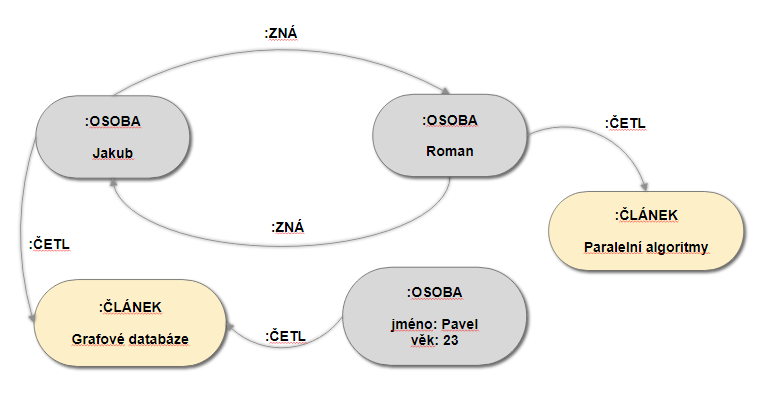
\includegraphics[width=12cm]{figures/labeled_graph}
\caption{Ohodnocený graf}
\label{fig:labeled_graf}
\end{center}
\end{figure}

% Property grafy
Ohodnocené grafy sice poskytují možnost rozlišit typy hran a uzlů, v mnoha situacích je ale žádoucí zachytit do grafu více informací. \textit{Atributové grafy} umožňují přiřadit hranám a uzlům libovolný počet atributů (dvojic klíč-hodnota), které obsahují informace o daném uzlu, respektive hraně. Příkladem může být věk osob, či datum vydání článku (viz obrázek \ref{fig:property_graf}). Většina grafových databází pracuje právě s atributovými grafy.\cite{Lal15}

\begin{figure}
\begin{center}
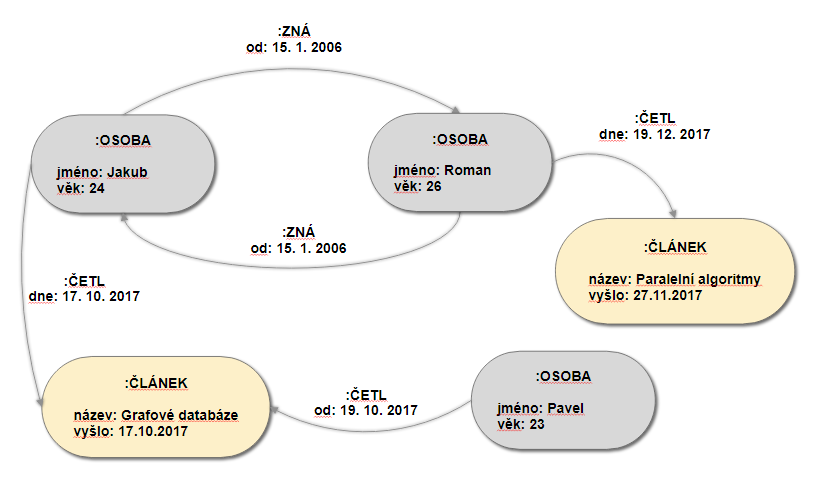
\includegraphics[width=12cm]{figures/property_graph}
\caption{Atributový graf}
\label{fig:property_graf}
\end{center}
\end{figure}

% Hypergrafy
Generalizací grafu je tzv. \textit{hypergraf}. Ten se proti grafu liší tím, že zatímco hrana grafu vede mezi právě dvěma vrcholy, hyperhrana (tedy hrana v hypergrafu) je mnoužinou jednoho a více vrcholů.\cite{Diestel00} Hypergrafy jsou používány k reprezentaci dat v mnoha oborech a některé grafové databáze je přímo podporují (například HypergraphDB\footnote{\url{http://hypergraphdb.org/}}).


\subsection{Reprezentace grafu}
\label{sec:gdb-reprezentace}
Aby bylo možné v dalších kapitolách popsat pokročilé aspekty grafových databází (jako jsou dotazování, indexování, či transakce v grafových databázích), je nejdříve nutné popsat jejich základní principy. Nutnost ukládat data ve formě grafů je starší než grafové databáze samotné, existuje tak mnoho způsobů uložení grafů z nichž ty nejběžnější zde popíšeme. Ještě předtím je nutno poznamenat, k jakým typům úloh jsou grafové databáze zejména využívány. Základními grafovými úlohami jsou \nomExpl{BSF}{průchod grafu do hloubky (Breadth-first search)} a \nomExpl{DFS}{průchod grafu do šířky (Depth-first search)}. Oba tyto algoritmy musí projít v nejhorším případě\footnote{Pro konkrétní problémy jsou často BFS a DFS algoritmy upravovány tak, aby bylo možné některé větve průchodu tzv. ořezávat - tedy procházet pouze jejich část, nebo je neprocházet vůbec.} všechny hrany a uzly grafu, je tedy vidět, že pro efektivitu grafových databází je klíčová rychlost přechodu z jednodoho uzlu do (všech) jeho sousedních uzlů pomocí existujících hran.

% RDBMS reprezentace
Než se pustíme do popisu nativních grafových uložišť, krátce popíšeme možnost ukládání grafů pomocí relačních databází. Jedním z možných řešení může být dvojice tabulek \textit{UZLY} a \textit{HRANY}. Tabulka uzlů by obsahovala identifikátor uzlu a případné další parametry uzlu, tabulka hrany by obsahovala referenci na počáteční a koncový uzel hrany a případné další parametry hrany\footnote{V tomto případě předpokládáme orientovaný prostý atributový graf, pro jiné grafy by bylo nutné tuto strukturu upravit (což ale není těžké). Například v případě ohodnoceného grafu je možné uvažovat separátní tabulku pro každý typ uzlů.}. Všechny hrany daného uzlu je tedy možné získat pomocí spojení těchto tabulek pomocí cízího klíče, složitější průchody potom mohou být docíleny pomocí relace tabulky hran na sebe sama. Problém tohoto přístupu je nutnost rekurzivních operací \textit{join} a jejich vysokých nákladů\footnote{Spojování tabulek pomocí cizích klíčů je jedna z nejdražších operací ve světě relačních databází.}. Tyto problémy mohou být částečně eliminovány použitím sloupcových či dokumentových NoSQL databází. Přestože v takovém případě nejsou používány rekurzivní operace spojování tabulek (ve světě NoSQL tato operace neexistuje), je k datům přistupováno pomocí prohledávání indexů a operace je tak stále výrazně dražší, než při použití nativního grafového uložiště.\cite{Lal15}

% Matice sousednosti
Nejzákladnější nativní reprezentací grafu je tzv. \textbf{matice sousednosti}. Ta využívá možnosti reprezentování hran grafu jako dvojice uzlů a reprezentuje graf jako matici \textit{M} o rozměrech \textit{|V|x|V|}, kde \textit{|V|} je počet uzlů grafu. Pokud existuje mezi uzly \textit{i} a \textit{j} hrana, pak bude \textit{M\textsubscript{i,j} $\neq$ 0}.
Pokud nás zajímá pouze existence hrany, nabývá matice pouze hodnot \textit{\{0, 1\}}. Pokud jsou hrany ohodnocené, pak nenulová hodnota buňky na dané pozici ukazuje nejen existenci hrany mezi danými uzly, ale také její ohodnocení. Pro neorientovaný graf je matice symetrická. Pokud je graf orientovaný, potom \textit{M\textsubscript{i,j}} určuje existenci hrany z uzlu \textit{i} do uzlu \textit{j} a \textit{M\textsubscript{j,i}} naopak existenci hrany z uzlu \textit{j} do uzlu \textit{i}.
Tato reprezentace grafu zajišťuje vysokou efektivitu přidávání, odstraňování a kontroly existence hran - tyto operace jsou okamžité.  Na druhou stranu přidání nového uzlu do grafu je nákladná operace, matice musí být přealokována a překopírována. Vzhledem k tomu, že paměťová náročnost matice sousednosti je kvadratická vzhledem k počtu uzlů a nezávisle na počtu hran (není tedy vhodná pro řídké matice\footnote{Poznamenejme, že matice reprezentující graf jsou často řídké, jedná se o grafy, kde je na velký počet uzlů poměrně málo hran, příkladem mohou být sociální sítě.}), je drahé i její překopírování.
Pro nalezení všech sousedních uzlů je nutné všechny uzly projít a zkontrolovat, zda hrana existuje, či nikoliv. Hledání sousedních uzlů je nejčastější operací při průchodu grafu, tato reprezentace tedy není vhodná ani na složitější průchody.

% Laplaceovská matice
Speciální variantou matice sousednosti je \textbf{Laplaceovská matice}. Ta má stejně jako matice sousednosti rozměry \textit{|V|x|V|}. Diagonála Laplaceovské matice ukazuje stupeň vrcholu a pokud existuje mezi dvěmi vrcholy hrana, je hodnota matice na dané pozici \textit{-1}. Pokud mezi vrcholy hrana není, hodnota je \textit{0}. Hlavní výhodnou reprezentace grafu Laplaceovskou maticí je umožňění spektrální analýzy grafu\cite{Barnard93}, kdy jsou pomocí vlastních čísel matice analyzovány vlastnosti grafu.

% Matice incidence
Další možnou maticovou reprezentací grafu je \textbf{matice incidence}. Jedná se o dvoudimenzionální matici o rozměrech \textit{|V|x|E|}, kde každý sloupec matice odpovídá jedné hraně a řádek jednomu uzlu. Pokud je uzel \textit{v} účastníkem hrany \textit{e}, potom \textit{M\textsubscript{v,e} != 0}. Pokud se jedná o neorientované grafy, nabývá matice pouze hodnot \textit{\{0, 1\}}. Pokud je graf orientovaný, potom je odchozí hrana kódována jako \textit{-1} a příchozí jako \textit{1}. V případě ohodnoceného grafu mohou být hodnoty obecně všechna celá čísla (podobně jako u matice sousednosti), přičemž opět platí, že záporné číslo značí odchozí hranu a kládné číslo příchozí. Vzhledem k tomu, že pro většinu grafů platí, že počet hran \textit{|E|} je vyšší než počet uzlů \textit{|V|} (často, například u sociálních sítí, je výrazně vyšší), je tato reprezentace pro svou vysokou paměťovou náročnost ve většině případů nevhodná. Narozdíl od ostatních reprezentací ale umožňuje ukládání hypergrafů (hrany hypergrafu mohou zahrnovat libovolný počet vrcholů). Zatímco u běžného grafu by každý sloupec matice incidence obsahoval právě dva nenulové prvky, u hypergrafu jich může být libovolný počet.

% List sousednosti
Některé problémy matice sousednosti řeší \textbf{list sousednosti}. Ten je implementován jako množina listů, kde každému uzlu připadá jeden list sousedních uzlů. Paměťová náročnost této reprezentace je tedy \textit{|V|+|E|}, kde \textit{|V|} je počet uzlů a tedy počet listů sousednosti a \textit{|E|} je počet hran a tedy celkový počet prvků obsažených v listech sousednosti. List sousednosti je výrazně úspornější reprezentací grafu z paměťového hlediska než je matice sousednosti a je tedy vhodný i pro řídké grafy. Zároveň umožňuje rychlé nalezení všech sousedních uzlů pro daný uzel, v listu jsou vypsány pouze ty uzly, se kterými je uzel propojen a procházení grafu je tak rychlé. Přidání hrany do grafu je přidáním jednoho prvku do listu (respektive dvou listů v případě neorientovaného grafu) a přidání uzlu je také relativně efektivní - znamená vytvoření nového listu a přidání ho do množiny ostatních listů. Drahé jsou naopak operace odebrání hrany (je nutné projít všechny sousedy obou koncových uzlů hrany) a odebrání uzlu (je nutné projít všechny hrany). Také ověření existence konkrétní hrany je relativně drahé (je potřeba opět projít všechny sousedy daného uzlu). Toto může být řešeno alternativní implementací, napříkald mohou být listy sousedů řazeny. Tím se sice sníží složitost ověření existence hrany, ale zvýší se složitost přidání nové hrany.
Při reprezentaci velkých grafů pomocí listů sousednosti se používají kompresní techniky, díky kterým je možné dále snižovat paměťovou náročnost.\cite{Boldi04} Jednotlivé reprezentace jsou ukázány na obrázku \ref{fig:reprezentace}.

\begin{figure}
\begin{center}
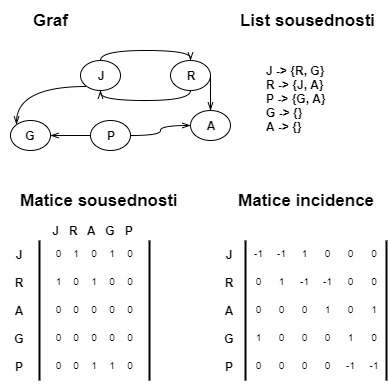
\includegraphics[width=8cm]{figures/graph_reprezentation}
\caption{Reprezentace (orientovaného) grafu}
\label{fig:reprezentace}
\end{center}
\end{figure}

Důležitým kritériem pro výběr reprezentace grafu je \textit{lokalita dat}. Cílem je uložit graf tak, aby jejich fyzické umístění odpovídalo jejich logické vzdálenosti a při průchodu grafem tak byla data pro další krok načtena co nejrychleji. K dosažení optimality lokality dat reprezentovaných grafem existuje mnoho technik, vzhledem k tomu, že se ale jedná o \textit{NP-těžkou} úlohu, jedná se často o heuristiky a aproximační algoritmy. Některé z používaných metod jsou například metoda minimalizace šířky matice autorů \textit{Cuthill a McKee} \cite{Cuthill69}, \textit{rekurzivní spektrální bisekce} \cite{Barnard93}, nebo metoda založená na průchodedech grafu do šířky (\textit{Breadth First Search Layout}) \cite{Furaih98}.


\subsection{Typy dotazů}
\label{sec:gdb-dotazy}

% Traversal pattern
Na rozdíl od indexově náročných množinových operací relačních databází využívají grafové databáze bezindexové místní prohledávání (traverzování) \cite{Anglels08}. Relační databáze obsahují data typicky v normalizované formě v několika separátních tabulkách tak, aby bylo zamezeno duplikaci dat. Řádky těchto tabulek mohou být chápány jako objekty popsané svými vlastnostmi. Vztahy mezi objekty jsou definovány primárními a cizími klíči a musí být při dotazování explicitně vytvořeny spojením tabulek pomocí \textit{join} operace. Jak vyhledávání záznamů v tabulkách, tak spojování tabulek je (v ideálním případě) realizováno pomocí vyhledávacích indexů, které časovou složitost těchto operací značně snižují, obecně ale ne dostatečně. Databázové vyhledávací indexy jsou typicky realizovány pomocí vyhledávacích stromů (konkrétně B-stromů \cite{Leach05}), vyhledání zánamu má tedy logaritmickou časovou složitost vzhledem k počtu uzlů\footnote{Konkrétně operaci vyhledání uzlu má složitost \textit{$\Theta$(b log$_b$(n))} a operace vyhledání rozsahu uzlů \textit{$\Theta$(b log$_b$(n) + k/b)}, kde \textit{n} je počet uzlů, \textit{b} je úroveň stromu a \textit{k} je velikost rozsahu.\cite{Cormen09}}.
Grafové databáze na druhé straně obsahují typicky pouze jednu strukturu - graf\footnote{Grafové databáže mohou obsahovat jeden velký graf, nesouvislý graf, nebo množinu grafů. Z hlediska této práce je toto ale technický detail a pokud nebude explicitně řečeno jinak, budeme předpokládat, že grafová databáze obsahuje jeden velký graf.}. Ten ve své fyzické reprezentaci obsahuje všechny své hrany, vztahy mezi objekty (vrcholy) v grafu jsou tedy implicitní, není potřeba je při každém dotazu vytvářet. Tato skutečnost s sebou nese výhody i nevýhody. Jednou z podstatných nevýhod je složitost rozdělení grafu na podgrafy a tedy obtížná distribuce grafu (popsáno v kapitole \ref{sec:gdb-distribution}). Naopak výhodou je instantní čas, ve kterém je možné se v grafu posouvat mezi sousedními uzly. To je natolik výraznou vlastnostní grafových databází, že výrazně ovlivňuje způsob, jakým je přistupováno k datům v grafových databázích. Tím nejčastějším je právě průchod grafem (traverzování, nebo také \textit{Traversal pattern}).

Na začátku průchodu grafu jsou pomocí indexu vyhledány výchozí uzly, ze kterých bude graf procházen. Z nich se dotaz pohybuje po grafu pomocí sousedních hran a uzlů dle zadaných kritérií. Těmi jsou typicky typy hran a uzlů, podmínky na jejich vlastnosti (uvažujeme atributový graf, viz kapitola \ref{sec:gdb-grafy}) a hloubka prohledávání. Součástí definice dotazu je také zvolení typu průchodu - průchod do hloubky (\textit{\nom{DFS}{Depth-first search}}, nebo průchod do šířky (\textit{\nom{BFS}{Breadth-first search}}. Když jsou projity všechny cesty odpovídající zadaným kritériím, jsou vráceny uzly, ve kterých průchod skončil. Typickými úlohami řešenými pomocí průchodů grafem je například zjištění existence cesty mezi dvěma uzly, nalezení nejktraší cesty, nalezení všech cest a uzlů odpovídajícíh zadaným kritériím apod. Na obrázku \ref{fig:traversal} je ukázán průchod, který by odpovídal na otázku "Co čtou přátelé lidí, kteří čtou stejný článek jako Pavel".

\begin{figure}
\begin{center}
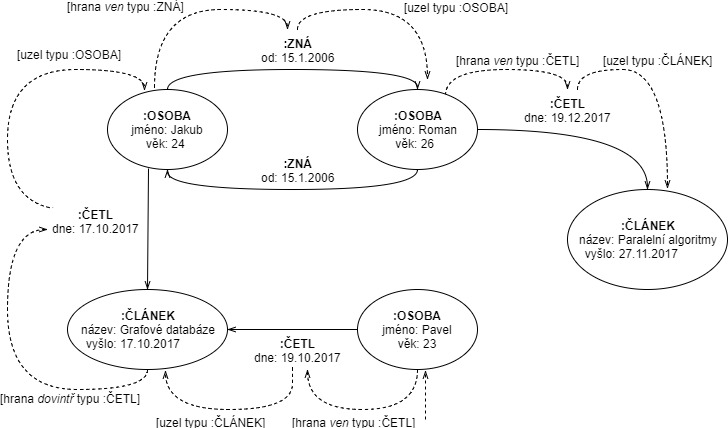
\includegraphics[width=14cm]{figures/traversal}
\caption{Příklad průchodu (\textit{traverzování} grafem)}
\label{fig:traversal}
\end{center}
\end{figure}

% Dotazy na podgraf, nadgraf, podobný graf
Dalšími typy dotazou kromě obecného průchodu gravu jsou \textit{dotazy na podgrafy}, \textit{dotazy na nadgrafy} a \textit{dotazy na podobné grafy}. Zadáním těchto dotazů je také graf, označme \textit{$G_\mathrm{dotaz}$}. Tento dotazový graf může obsahovat uzly a hrany, u kterých nejsou specifikovány bližší vlastnosti, v grafu může být určena množina přípustných typů uzlů a hran, nebo například maska jejich typů. Dotazy na podgrafy hledají specifický vzor grafů v grafové databázi - v databázi jsou vyhledávány všechny grafy, který \textit{$G_\mathrm{dotaz}$} obsahují. V případě dotazu na nadgraf naopak hledáme v databázi všechny datové grafy, které jsou v \textit{$G_\mathrm{dotaz}$} obsaženy. U dotazů na podobné grafy je výsledek dotazu vyhodnocován pomocí metriky podobnosti.\cite{Koutra11} Tyto typy dotazů jsou vyhodnocovány ve třech krocích:

\begin{enumerate}
	\item{Extrakce:} Z grafu \textit{$G_\mathrm{dotaz}$} jsou vyextrahovány indexované charekteristiky (stejným způsobem jako z datových grafů).
	\item{Filtrace:} Porovnáním vyextrahovaných charakteristik jsou z datových grafů vybrány ty, které odpovídají charakteristikám \textit{$G_\mathrm{dotaz}$}. Tím vznikne množina kandidátů na výsledek, přičemž cílem indexační techniky je, aby tato množina obsahovala co nejmenší počet falešně pozitivních kandidátů. Pokud by množina neobsahovala žádné falešně pozitivní kandidáty (indexační technika by měla dostatečnou filtrační schopnost), byla by tato množina rovna množině výsledných grafů (a nebylo by nutno provádět třetí fázi).
	\item{Verifikace:} Grafy z množiny kandidátních řešení jsou podrobně porovnány s \textit{$G_\mathrm{dotaz}$}, čímž jsou vyloučeni případní zbylí falšeně pozivní kandidáti a dostáváme množinu skutečných výsledků.
\end{enumerate}

Je zjevné, že tyto typy dotazů jsou velmi závislé na konkrétních indexačních technikách, ty jsou popsány v kapitole \ref{sec:gdb-indexy}. Grafické znázornění dotazů na nadgraf a podgraf je na obrázku \ref{fig:supergraph_subgraph_query}.

\begin{figure}
\begin{center}
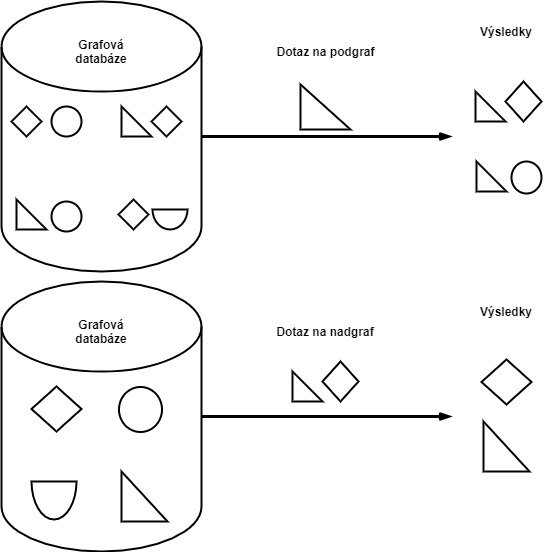
\includegraphics[width=10cm]{figures/supergraph_subgraph_query}
\caption{Znázornění dotazů na nadgraf a podgraf}
\label{fig:supergraph_subgraph_query}
\end{center}
\end{figure}

\subsection{Indexy}
\label{sec:gdb-indexy}
% Indexování uzlů a hran
Stejně jako je tomu u relačních databází, i ve světě grafových databází se hojně používají indexy (a také už byly v předchozím textu několikrát zmíněny) a je jich hned několik typů. Průchody (\textit{traverzování}) grafem používají pouze základní indexy a to ve chvíly, kdy jsou hledány výchozí uzly. Konkrétní databáze můžou k indexům přistupovat specifickým způsobem, je tedy vhodné si u každé databáze ověřit, co je automaticky indexováno. Zpravidla je žádoucí indexovat typy (\textit{labely}) a vybrané atributy hran a uzlů. Například pokud by existoval index na typ uzlů a chtěli bychom v grafu o milionu uzlů vyhledat všechny uzly typu \textit{:OSOBA} (a z nich graf procházet), databáze by neprocházela všechny uzly, ale podle indexu by vyhledala přesně uzly tohoto typu. Tyto základní indexy si můžeme představit jako indexy které známe z relačních databází, tedy jako B-stromy a jim podobné struktury\footnote{Implementace indexu v Neo4J (\textit{GB+Tree}): \url{https://github.com/neo4j/neo4j/blob/3.4/community/index/src/main/java/org/neo4j/index/internal/gbptree/GBPTree.java}}.

% indexační metody pro dotazy na podgraf (mining a non-mining based), nadgraf a podobný graf
U strukturálních dotazů je situace komplikovanější. V případě \textit{dotazů na podgrafy} se indexační metody dělí na tzv. \textit{mining based} (indexy založené na dolování dat (\textit{data mining})) a \textit{non-mining based}. \textit{Mining based} indexační metody jsou založené na pozorování, že pokud množina vlastností grafu \textit{$G_\mathrm{dotaz}$} není obsažena v některém z datových grafů, nebude takový datový graf obsahovat ani celý dotazový graf. Stačí tedy vybrat vhodné podstruktury grafu \textit{$G_\mathrm{dotaz}$} a vyhodnocovat dotazy pouze na nich (typicky se jedná o časté podstromy či podgrafy). Pro tyto podmnožiny vlastností je vytvořen \textit{invertovaný index}\footnote{Invertovaný index ukazuje pro všechny hodnoty seznam celků, v kterých je hodnota obsažena, v tomto případě tedy pro všechny podstruktury ukazuje v kterých datových grafech jsou obsaženy.} a při vyhodnocování grafu \textit{$G_\mathrm{dotaz}$} jsou nejdříve identifikovány a vyhodnoceny tyto struktury, čímž je získána množina kandidátů. Nevýhodou tohoto přístupu je závislost \textit{invertovaného indexu} na jak datových, tak dotazových datech. Pokud se výrazně změní typ dotazových grafů, nebo se změní datové grafy tak, že vybrané podstruktury již nemají potřebnou filtrační schopnost, je nutné přeindexovat. Mezi \textit{mining based} indexační metody patří například \textit{GIndex} \cite{Yan04} a \textit{TreePI} \cite{Zhang07}. \textit{Non-mining based} indexační metody naopak indexují grafy jako celek, neanalyzují jejich strukturu nabo časté vzory. Nejsou tak závislé na dotazových ani datových grafech, nedosahují ovšem takové filtrační schopnosti jako \textit{mining based} metody a tím pádem vyžadují delší fázi verifikace. Patří mezi ně \textit{GraphGrep} \cite{Giugno02}, \textit{GDIndex} \cite{Williams07}, \textit{GString} \cite{Jiang07} a \textit{GraphREL} \cite{Sakr09}. Narozdíl od \textit{dotazů na podgrafu} neexistuje pro \textit{dotazy na podgrafy} zatím tolik indexačních technik (a to i přesto, že se jedná o důležitý problém), mezi existující patří \textit{cIndex} \cite{Chen07}, \textit{GPTree} \cite{Zhang09} a \textit{iGQ} \cite{Wang16}. U \textit{dotazů na podobné grafy} je cílem nalézt grafy, které jsou dotazovému grafu \textit{$G_\mathrm{dotaz}$} podobné, je tedy nutné určit metriku, podle které bude podobnost měřena. Indexačními metodami pro tuto oblast jsou \textit{Grafil} \cite{Yan05}, \textit{Closure Tree} \cite{He06} a \textit{SAGA} \cite{Tian07}.

% TODO fultextové indexy + intervalové hledání - LUCENE

\subsection{Transakce}
%ACID
Pojďme nejprve připomenout standardní transakční model světa relačních databází - \textbf{ACID}. Tento model říká, že transakce v databázovém systému musí být atomické (\textit{\textbf{A}tomocity}, tedy nedělitelné. Pokud tedy selže některá z operací transakce, selže celá transakce a je proved její \textit{rollback}\footnote{Rollback transakce je událost, která nastává, pokud transakce selže, nebo pokud je uživatelem explicitně vyvolána. Všechny kroky, které byly v rámci transakce provedeny jsou vráceny, po rollbacku transakce je tedy databáze ve stejném stavu, jako před spuštěním transakce. Opakem rollbacku je operace \textit{commit}, která potvrzuje všechny změny provedené v transakci.}. Nemůže se tedy stát, že by byla provedena jen část operací transakce a databáze se ocitla v nekonzistentním stavu. Jinými slovy, po provedení jakékoliv transakce (úspěšném i neúspěšném) bude databáze vždy konzistentní (\textit{\textbf{C}onsistency}). Všechny transakce jsou také izolované (\textit{\textbf{I}solated}), tedy transakce jsou na sobě navzájem nezávislé a neovlivňují si navzájem data. V případě, že dojde ke konfliktu několika transakcí, databázový systém konflikt vyřeší tak, aby byla tato vlastnost zachována\footnote{Existuje několik stupňů izolace transakcí , výčtem \textit{read uncommitted}, \textit{read committed}, \textit{repeatable read} a \textit{serializable}.}. Právě na úrovni izolace konfliktujících transakcí záleží, jakým způsobem bude konflikt vyřešen. Poslední vlastností transakcí v transakčním modelu ACID je trvanlivost (\textit{\textbf{D}urability}). Tato vlastnost zajistí, že změny provedené transakcí jsou trvalé.

%BASE
Vlastnosti ACID transakčního modelu jsou klíčové pro relační databázové systémy, které mají širokou škálu využití. Pro svět NoSQL databází (do kterého bývají grafové databáze často řazeny) tento model ale není vhodný, a to především kvůli silnému důrazu na konzistenci dat a tedy jejich obtížné distribuovatelnosti\footnote{Distribuovanost dat je klíčová pro NoSQL databáze obecně, pro grafové databáze to ale ne vždy platí. Toto bude více rozebráno v kapitole \ref{sec:gdb-distribution}.}. Zaven je tedy alternativní transakční model - \textbf{BASE}. Ten říká, že systém numusí být nutně dostupný vždy, stačí základní dostupnost (\textit{\textbf{B}asic \textbf{A}vailability}) - tedy dostupnost po většinu času. Mohou nastastat částečné výpadky, ale nikdy nedojde k výpadku celého systému. Tato vlastnost se opět týká především těch NoSQL databází, které předpokládají vysokou distribuovanost dat a skládají se z mnoha uzlů. Od grafových databází, které distribuované nejsou očekáváme tedy dostupnost úplnou. Systém je v takzvaném volném stavu (\textit{\textbf{S}oft-state}), je dynamický, neustále docházi ke změnám. V případě distribuování a replikaci dat je důsledkem této vlastnosti mimo jiné to, že ne všechny repliky musí být nutně vzájemně konzistentní. A konečně, máme jistotu, že systém bude vždy "nakonec" uveden do konzistentního stavu (\textit{\textbf{E}ventual consistency}), ale nemusí být konzistentní v každém okamžiku. Například k vynucení konzistence může dojít až při čtení dat, při jejich zápisu nutná není. Tento model tedy také umožňuje zachování jistoty konzistence dat, není ale automatická, jako tomu je u předchozího modelu. \cite{Sadalage13}

Jak už bylo zmíněno, grafové databáze jsou typem NoSQL databází. Přesto většina grafových databází není NoSQL databází v pravém smyslu slova. Výsledkem tak je, že některé grafové databáze plně podporují ACID transakční model, jiné naopak BASE. Toto je blíže diskutováno v popisu konkrétních grafových databází (kapitola \ref{sec:gdb-databaze}).

\subsection{Distribuovatelnost}
\label{sec:gdb-distribution}
V kapitole \ref{sec:gdb-nosql} jsme zmínili, že distribuovanost dat je klíčovou vlastností NoSQL databází\footnote{Pokud je to možné, je vždy efektivnější když data distribuovaná nejsou. K jejich distribuování přikračujeme až ve chvíli, kdy nás k tomu nutí okolnosti - například velikost dat.}. Pro distribuci dat se využívá kombinování dvou technik - \textit{rozdělení (sharding)} a \textit{replikace} dat.

% Sharding
Rozdělení dat je základním předpokladem pro jejich distribuci - musí dojít k rozdělení dat na vhodné množiny a ty uložit na různé uzly v clusteru. Při manipulaci s daty je tak přistopováno na jeden nebo více uzlů podle toho, jaká data jsou zpracovávána. Při rozdělování dat je bráno v potaz jejich rovnoměrné rozdělení, minimalizace počtu uzlů využívaných k provádění operací nad daty a optimalizace jejich fyzického rozmístění.

% Replikace
Aby byla při případném výpadku části uzlů stále přístapná všechna data (všechny \textit{shardy}) jsou po částech mezi uzly několikrát replikována. Tím je zajištěno, že při selhání (ať už dočasném, nebo trvalém) jednoho uzlu nedojde ke ztrátě dat samotných, ani ke ztrátě přístupu k nim (pokud neselžou všechny repliky obsahující danou část dat). Počet, kolikrát jsou data v databázi replikována (replikační faktor) určuje mimo jiné algoritmus, pomocí kterého jsou data na repliky ukládána a rychlost jejich čtení.

% Kontext grafů
U grafových databází je ale distribuce dat (a tedy horizontální škálování) výrazně komplikovanější, než u ostatních NoSQL databází. Data v nich jsou uložena do několika několika struktur (tabulek, dokumentů, dvojic klíč-hodnota), zatímco obsahem grafové databáze je typicky pouze jediná struktura - graf. Rozdělení grafu na podgrafy je obtížný problém (zvláště pokud se jedná například o úplný graf), proto obecně ne mnoho grafových databází tuto možnost vůbec umožňuje. Přesto existují metody, které se distribucí grafu zabývají. Výsledná distribuce je potom optimální pouze pro podmnožinu grafových úloh (například průchod do šířky, hledání nejmenší kostry atd.). Distribucí grafu na několik uzlů se mění čas, v jakém je možné získat seznam sousedních vrcholů grafu v případech, kdy hrana mezi vrcholem a jeho sousedem spojuje dva podgrafy na dvou různých uzlech, je tedy obtížné graf distribuovat při snaze zachovat co nejvyšší rychlost průchodu grafem. Příkladem algoritmů pro rozdělení grafu může být \textit{1D dělení} a \textit{2D dělení} matice sousednosti \cite{Yoo05}, nebo mnoho technik aproximujících \textit{optimální k-rozdělení grafu}\footnote{Optimální bisekce grafu je NP-obtížný problém \cite{Garey90}, tedy i optimální k-rozdělení grafu je nejméně NP-obtížný problém. Proto jsou používány aproximační algoritmy.}.\cite{George78} \cite{Fiduccia82} \cite{Battiti99}

\subsection{Databáze - příklady}
\label{sec:gdb-databaze}

% Neo4J
V této sekci popíšeme vlastnosti několika nejpoužívanějších grafových databází (relevantních pro projekt \textit{Manta Tools} a tedy i tuto diplomovou práci). Dlouhodobě nejoblíbenější grafovou databázi na trhu \cite{Ranking17} je \textbf{Neo4j}\footnote{\url{https://neo4j.com/}} Databáze je implementovaná v programovacím jazyku \textit{Java}, má \textit{nativní grafové uložiště}, nabízí \textit{horizontální škálovatelnost} a také plnohodnotný \textit{ACID transakční model}. Dotazování dat můžebýt prováděno pomocí objektového \textit{Java API}, nebo jazyků \textit{Cypher} a \textit{Gremlin} (viz \ref{sec:gdb-jazyky}).
Databáze \textit{Neo4j} je licencována pod \textit{GPLv3}\footnote{\url{https://www.gnu.org/licenses/gpl-3.0.en.html}} licencí.

% OrientDB (a ArangoDB)
Další oblíbená databáze, \textbf{OrientDB}\footnote{\url{http://orientdb.com/}} podporuje hned několik způsobů práce s daty - může být používána jako databáze grafová, dokumentová, objektová, nebo databáze typu klič-hodnota (označuje se jako \textit{multi-modelová}) \cite{OrientMultiModel}. Uzly grafů jsou reprezentovány jako (\textit{JSON}) dokumenty, hrany mohou být buďto také dokumenty(\textit{regular}), nebo mohou být pouze parametrem uzlů (\textit{lightweight}). Nejedná se tedy o \textit{nativní reprezentaci grafu}, jak je popsána v kapitole \ref{sec:gdb-reprezentace}.
Stejně jako \textit{Neo4j} je i \textit{OrientDB} implementovaná v programovacím jazyce \textit{Java} a umožňuje \textit{horizontální škálování}. Výchozím transakčním modelem je \textit{ACID}, od verze \textit{2.1.7} je ale možná konfigurace transakčního modelu \textit{BASE} ve dvou režimech řešení kolizí \cite{OrientConsistency}, což má pozitivní dopady na rychlost databáze. S databází je možné komunikovat pomocí \textit{HTTP REST/JSON API}, \textit{Java API} a jazyka \textit{Gremlin}. Krom těchto možností nabízí \textit{OrientDB} ještě vlastní dialekt jazyk \textit{SQL}. Licenční politika je více přívětivá komerčnímu použití než je tomu u \textit{Neo4j}, \textit{OrientDB} je licencováno pod \textit{Apache 2.0}\footnote{\url{https://www.apache.org/licenses/LICENSE-2.0}} licencí.
Databází s velice podobonými charakteristikami jako má \textit{OrientDB} je \textbf{ArangoDB}\footnote{\url{https://www.arangodb.com/}}, hlavním rozdílem je, že jádro \textit{ArangoDB} je implementováno v \textit{C++} a dle vlastních testů \cite{ArangoBenchmark} je (zvláště pro některé typy úloh) výrazně efektivnější.

% Titan (a JanusGraph)
\textbf{Titan} se oproti předchozím databázím výrazně liší, nejedná se plnohodnotnou databázi s vlastním uložištěm, ale "pouze" a softwarovou mezivrstvu, která poskytuje funkcionalitu grafových databází jako nadstavbu nad jinými \textit{NoSQL} databázemi. Těmi jsou \textit{Apache Cassandra}\footnote{\url{http://cassandra.apache.org/}}, \textit{Apache HBase}\footnote{\url{http://hbase.apache.org/}} a \textit{Oracle BerkeleyDB}\footnote{\url{http://www.oracle.com/technetwork/database/database-technologies/berkeleydb}}.
\textit{Titan} je zaměřen (jak už napovídají nabízené \textit{back-end} databáze) na masivní škálovatelnost grafových databází, zároveň ale nabízí oba transakční modely - \textit{ACID} i \textit{BASE}. Dotazování dat v Titanu je možné pomocí \textit{Java API}, nebo jazyka \textit{Gremlin}. V roce 2015 proběhla akvizice \textit{Titanu} (respektive společnosti \textit{Aurelius}, která ho vyvíjela) společností \textit{DataStax}, čímž prakticky skončil vývoj této databáze. \textit{Open-source forkem} a pokračovatelem\cite{Datami17} \textbf{Titanu} je databáze \textit{JanusGraph}\footnote{\url{http://janusgraph.org/}}. Obě databáze jsou implementovány v programovacím jazyce \textit{Java} a licencovány pod \textit{Apache 2.0} licencí.


\subsection{Dotazovací jazyky}
\label{sec:gdb-jazyky}

% API a REST API
Do roku 2018 nebyly zatím definovány standardy pro dotazování dat v grafových databázích. Existuje mnoho způsobů a nástrojů, které dotazování dat umožňují, většina z nich je ale spjata s konkrétní databází. Některé dotazovací jazyky jsou sice již podporovány více databázemi, v podstatě žádný ale zatím nelze prohlásit za obecně používaný standard. Základním způsobem dotazování dat v kontextu grafových databází jsou \textit{programová rozhraní}, nebo případně \textit{REST API} nezávislá na konkrétním programovacím jazyku. Jednoznačnou výhodou tohoto přístupu je, že tato API, která má každá grafová databáze své, podporují všechny funkce dané databáze. To je zároveň i hlávní nevýhodou - grafové databáze fungují na různých, často protichůdných principech (např. tranasakční a netransakční databáze, distribuované a nedistribuované atd.), a jejich API se tedy liší. Není tedy možné předpokládat, že průchody grafem napsané pro jednu databázi budou fungovat na druhé\footnote{Toto zcela neplatí ani u SQL, které je jednoznačným standardem ve světě relačních databází. Rozdíl je ale v tom, že zatímco různé dialekty SQL se liší (pokud se liší) zpravidla pouze málo a pouze v syntaxi jazyka, u API různých grafových databází mohou být rozdíly mnohem zásadnější.}.

% deklarativní versus imperativní pattern
Tyto překážky v rozdílnosti grafových databází se snaží vyřešit hned několik dotazovacích jazyků, ty postupně vznikaly spolu s tím, jak se grafové databáze vyvíjely. Tyto jazyky lze dělit mnoha způsoby, jedním z nejdůležitějších je dělení na \textit{deklarativní} a \textit{imperativní}. Zatímco \textit{imperativní} jazyky formulují řešení problému pomocí pousloupnosti příkazů a určují tak přesný algoritmus řešení problémů, \textit{deklarativní} jazyky naopak způsob řešení problému nepopisují vůbec, ale soustředí se na popis požadovaného výsledku - deklarují, jaký má být výsledek (použitý algoritmus tedy určuje interpret daného jazyka).\cite{Chao16}

% Gremlin
Jedním z nejpoužívanějších grafových dotazovacích jazyků je \textbf{Gremlin}. První verze \textit{Gremlina} vyšla 25. 12. 2009 \cite{Gremlin09} jako součást \textit{open-source} projektu \textit{TinkerPop}. \textit{Gremlin} byl uveden jako \textit{turingovsky kompletní} programovací jazyk pro práci s atributovými grafovými databázemi. Umožňoval \textit{\nomExpl{CRUD}{Create Read Update Delete}} operace, různé způsoby průchodů grafem a operace s vyhledávacími indexy. V této verzi podporoval ze zavedených databází pouze databázi \textit{Neo4j}.
V roce 2010 bylo uvedeno rozhraní \textit{Blueprints} \cite{Blueprints10}, jehož implementací grafová databáze získává podporu jazyka \textit{Gremlin}.
Ve verzi \textit{Gremlina 2.6.0} \cite{Gremlin14} už jsou \textit{Blueprints} poměrně široce podporovány\footnote{Ve verzi \textit{2.6.0} \textit{Gremlin} podporují databáze \textit{Neo4j, OrientDB, Sparksee, Titan, Faunus, InfiniteGraph, Rexster,} a další.}. To je ale také poslední verze vydaná pod samostatným projektem \textit{TinkerPop}, poté se celý projekt stává součástí \textit{Apache software foundation}\footnote{\url{http://www.apache.org/}}.
To znamená několik změn v projektu, ve verzích \textit{3.x} \cite{Gremlin17} je pozměněna systaxe jazyka a také se mění \textit{API} pro podporu \textit{Gremlina} na \textit{Gremlin Structure API}. Od této verze podporuje \textit{Gremlin} také \textit{deklarativní} dotazování dat (do té doby byly všechny dotazy pouze \textit{imperativní}).  Mezi databáze podporující Gremlin \textit{3.x} patří \textit{Neo4j, DataStax, InfiniteGraph, JanusGraph, Cosmos DB} a další. V příkladu \ref{exa:gremlin} je ukázán průchod grafem v \textit{Java} notaci jazyka \textit{Gremlin}.

\lstinputlisting[language=Java, caption=Gremlin (Java) - průchod grafem, label=exa:gremlin]{code/GremlinTraversalExample.java}

% Cypher
Dalším velice oblíbeným dotazovacím jazykem je \textbf{Cypher} \cite{Cypher}, a to především díky jeho podobnosti s \textit{SQL}. \textit{Cypher} je \textit{deklarativní DSL jazyk}, který vznikl jako součást Neo4j. Vzhledem k tomu, že se jedná o \textit{deklarativní} jazyk, snaží se co nejčitelněji popsat\footnote{Syntaxe \textit{Cypheru} je inspirována syntaxí jazyka \textit{SQL} a také takzvaným \textit{ASCII artem} - \url{https://cs.wikipedia.org/wiki/ASCII_art}}, co má být výsledkem dotazu a naopak se zaměřuje na to, jakým způsobem bude dotaz proveden. Přesto je možné vykonávání dotazů ovlivnit pomocí tzv. \textit{hintů} (například lze ovlivnit použití indexů). \textit{Cypher} si získal mezi uživateli  značnou oblibu, vznikla proto iniciativa rozšířit ho i mezi další grafové databáze a pokusit se ustanovit \textit{Cypher} jako standardní dotazovací jazyk pro grafové databáze. Výsledkem této iniciativy byl vznik \textit{OpenCypheru} \cite{openCypher} v roce 2015. Podpora tohoto jazyku ale zatím není příliš široká.\footnote{\textit{OpenCypher} v tuto chvíli podporují spíše méně známé grafové databáze: \url{http://www.opencypher.org/projects}.} V příkladu \ref{exa:cypher} je ukázka \textit{Cypher} dotazu.

\lstinputlisting[language=Sql, caption=Ukázka Cypher dotazu, label=exa:cypher]{code/CypherQueryExample.sql}

Existují i další dotazovací jazyky pro grafové databáze než výše zmíněné, většina z nich je ale navržena pro specifické účely a pro obecné použití se nehodí, a nebo nejsou příliš rozšířené.


%%%%%%%%%%%%%%%%%%%%%%%%%%%%%%%%%%%%%%%%%%%%%%%%%
%%%%%%%%%%%%%%%%%%%%%%%%%%%%%%%%%%%%%%%%%%%%%%%%%
%%%%%%%%%%%%%%%%%%%%%%%%%%%%%%%%%%%%%%%%%%%%%%%%%
%%%%%%%%%%%%%%%%%%%%%%%%%%%%%%%%%%%%%%%%%%%%%%%%%
%%%%%%%%%%%%%%%%%%%%%%%%%%%%%%%%%%%%%%%%%%%%%%%%%
\section{Softwarové abstrakce}

% Důvody pro abstrakci abstrakce
Vývoj softwaru je dnes jistě v mnoha ohledech jednodušší, než v padesátých letech dvacátého století, kdy programátor musel znát strojový kód, počty a velikosti registrů a v nejhorších případech musel fyzicky propojit vodiče mezi výpočetními jednotkami. Postupem času s příchodem nových programovacích jazyků byl programátor stále více abstrahován od hardwaru a i některých softwarových vrstev nad ním. Vývojáři webových stránek stačí vhodný operační systém, aplikační a databázový server k tomu, aby mohl rychle vytvořit webové stránky, nepotřebuje k tomu přitom podrobnou znalost všech používaných technologií. Stejně tak Java vývojář dnes již nebude psát celou aplikaci s pomocí Javy samotné, ale využije mnoho existujících open-sourcových knihoven, které mu práci výrazně usnadní. Není tedy nutné, aby uměl vývojář vyřešit každý problém, pro řešení některých stačí přepoužití vhodných nástrojů. To má za následek nejen usnadnění práce při implementaci, ale také celkově čistší a přehlednější kód aplikace - kód obsahuje pouze aplikační logiku a nezbytné množství obslužných rutin. Přehledný kód potom vede k jednoduššímu vývoji, testování a údržbě aplikace. Lze tedy říci, že vhodně zvolené abstrakce na různých úrovních - ať už se jedná o architekturu celé aplikace, či návrh několika spolupracujících tříd, jsou pro softwarové systémy klíčové.

``Software je postaven na abstrakcích. Když vyberete ty správné, programování bude přirozeně vyplývat z návrhu, moduly budou mít minimalistická a jednoduchá rozhraní a nová funkcionalita bude dobře zapadat bez zásadních změn. Pokud vyberete špatné, programování bude řada ošklivých překvapení, rozhraní budou nucena vyhovět neočekávaným požadavkům, stanou se nemotorná a i nejjednodušší změna bude obtížně dosažitelná. Systém postavený na chybných konceptech nemůže zachránit žádné množství úprav, pouze jeho nové vytvoření od začátku.'' \cite{Jackson06}

% Od zapouzdření k API
Základním principem zajišťující abstrakci na úrovni zdrojového kódu aplikací je \textit{zapouzdření} - tedy princip, který říká, že stav objektů by neměl být přímo přístupný, ale mělo by k němu být přistupováno pomocí operací k tomu určených. Tím je zaručeno, že stav objektu bude upravovány pouze v rámci daných omezení (například viditelnost polí, číselný rozsah atd). Stejně tak je žádoucí, aby nebyla veřejně vystavována vnitřní implementace softwarových celků - tříd, knihoven, modulů, atd. Snažíme se tedy abstrahovat uživatele od toho, jak je takový celek vnitřně implementován a nabízíme mu pouze rozhraní pro práci s ním - API (\textit{Appplication Programming Interface}).

Cílem této kapitoly je popsat pro práci relevantní principy sloužící k zavedení vhodných úrovní softwarové abstrakce. Konkrétně popisuje API jako obecný nástroj k oddělení různých částí aplikace (kapitola \ref{sec:api}); vícevrstvou architekturu (kapitola \ref{sec:n-tier}), jejíž návrh pro definovaný problém je jedním z cílů této diplomocé práce; a architektonický styl \textit{REST} (kapitola \ref{sec:rest}), který je dnes jedním ze standardů pro architektury webových aplikací. Na závěr jsou popsány principy architektur určených pro \textit{cloudové} systémy (kapitola \ref{sec:cloud}). Ty jsou již několik let sílícím trendem a bylo by krátkozraké je nevzít v potaz.

\subsection{API}
\label{sec:api}
API je jasně definovaným rozhraním, které poskytuje uživateli přístup k funkcím softwarové jednotky, kterou obaluje. Vzhledem k tomu, že API je obecný pojem a má v softwarovém inženýrství široké uplatnění (které je v této kapitole alespoň částečně popsáno), neexistuje obecně uznávaná definice, která by vymezovala, z čeho se API skládá. Obecně je API souborem specifikací programových rutin a datových struktur.

% private/open API
Důležitou charakteristikou API je, zda se jedná o privátní, nebo veřejné API. \textit{Privátní API} je pouze technickým nástrojem pro modularizaci aplikace a přistupují k němu pouze jiné části aplikace. Takové API může být postupným vývojem aplikace upravováno bez dopadů na další (okolní) systémy. \textit{Veřejné API} naopak může být používáno mnoha různými spotřebiteli (v okamžik uveřejnění API poskytovatel často ztrácí kontrolu nad tím, kdo API používá), což má pro jeho charakteristiku několik dopadů. Tím nejdůležitějším je, že je velmi obtížné měnit jednotlivé části veřejného API - vždy existuje někdo, kdo je používá. Musí být tedy kladen ještě větší důraz na návrh a testování takového API. Speciálním případem veřejných API je \textit{SPI (Service Provider Interface)}, což je API poskytované bez implementace, ta je zajištěna třetími stranami.

% API types
API jsou používána na různých úrovních softwarové abstrakce. Nejblíže hardwaru jsou \textbf{lokální API} sloužící pro komunikaci mezi aplikacemi a různými vrstvami operačních systémů. Příkladem takového API je například \textit{POSIX} \cite{Posix} - rodina standardů, jejímž cílem je zajištění kompatibility mezi operačními systémy.

Na úrovni konkrétních programovacích jazyků jsou používána API sloužící jako rozhraní poskytující funkcionalitu softwarové knihovny (například \textit{Log4j}\footnote{\url{https://logging.apache.org/log4j/2.x/manual/api.html}}), frameworku (například \textit{Java Collections}\footnote{\url{https://docs.oracle.com/javase/tutorial/collections/}}), konrétní vrstvy či modulu aplikace. Zde neexistuje souhrné poujmenování, respektive, jako kategorie zde slouží programovací jazyky, pro které je API určeno - \textbf{Java API}, \textbf{Scala API}, atd. Tato API bývají často používána pro svou přímost, omezují ale své použití na prostředí homogenní z pohledu programovacího jazyka.

Spolu s rozvojem počítačových sítí a později také internetu vznikla poptávka po možnosti vzdáleného volání aplikací (nebo částí aplikací). Jedním z průkopníků v této obasti je \textit{RPC (Remote Procedure Call)}, technologie umožňující vykonání kódu, který je fyzicky na jiném zařízení, než volající program. Teoretické návrhy \textit{RPC} pochází ze sedmdesátých a první implementace z osmdesátých let dvacátého století. V roce 1998 se objevil soubor pravidel, který popisuje jak využívat technilogie RPC a XML k vzdálenému volání procedur přes internet - \textit{XML-RPC} \cite{Winner99}. XML poskytuje slovník pro popis RPC volání přenášená mezi počítači, technologie tak prakticky umožňuje vytváření API pro komunikaci dvou a více nehomogeních prostředí \cite{Laurent01}. Nástupcem \textit{XML-RPC} se stal \textit{SOAP}, který je postavený na podobných principech jako XML-RPC. Cílem \textit{SOAP}u je zajistit rozšířitelnost, neutralitu a nezávislost komunikace. Specifikace SOAPu byla zveřejněna v roce 1999, ale až verze 1.2 se v roce 2007 stala doporučením \textit{W3C}\footnote{https://www.w3.org/} \cite{W3C07}. Souběžně byl definován architektonický styl \textit{REST} (kapitola \ref{sec:rest}), který se \textit{SOAP}em několik let soutěžil o převahu a v současné době je \textit{de-facto} standardem pro architektury webových aplikace a tedy i \textbf{webových API}.

% vlastnosti dobrého API
Bez ohledu na účel, kterému API slouží, jeho návrh by se měl řídit několika obecnými pravidly \cite{Bloch06}. Dobré API by mělo:
\begin{itemize}
  \item{\textit{být snadno použitelné}}: API by mělo být intuitivní a funkcionalita poskytovaná API by měla být přístupná jednoduše. API by také mělo být minimální, tj. mít co nejméně veřejných prvnků a mělo by mít jasnou a svému účelu adekvátní jmennou konvenci. Takové API je jednoduché na pochopení, zapamatování a ladění.
  \item{\textit{být kompletní}}: API by mělo pokrývat veškerou předpokládanou funkcionalitu tak, aby nemuselo být pro nekomplenost nijak obcházeno. Toto je v konfliktu s principem minimality, obě vlastnosti musí být dobře vyváženy.
  \item{\textit{být rozšířitelné}}: API by mělo být možné v budoucnu rozšiřovat bez změn na stávající části API (veřejná, ale i privátní, API je velice komplikované zpětně upravit).
  \item{\textit{vést k čitelnému kódu}}: API by mělo umožnit psaní přehledného, čitelného a efektivního kódu. Naopak by jeho použití nemělo vést k nutnosti přidávání zbytečného kódu (\textit{boilerplate code}).
\end{itemize}

\subsection{Softwarové architektury}
\label{sec:architectures}
Softwarová architektura je úroveň návrhu softwaru, která sahá za hranice konkrétních algoritmů a datových struktur výpočtu. Navrhuje a specifikuje obecnou strukturu systému včetně komunikace,
synchronizace a přístupu k datům. Architektura přiřazuje funkcionalitu jednotlivým návrhovým elementům, předurčuje jejich fyzickou distribuci, kompozici, škálovatelnost, výkon a také jejich možné alternativy \cite{Garlan94}. Jádrem softwarové architektury je princip abstrakce - skrývání některých detailů pomocí zapouzdření za účelem lepší identifikace vlastností návrhových elementů \cite{Shaw90}. Komplexní systém může mít mnoho úrovní abstrakce a mnoho operačních fází, přičemž každá z nich může mít vlastní architekturu \cite{Bass98}.

Formálně jsou softwarové architektury popisovány pomocí konfigurací tzv. \textit{architektonických elementů} (\textit{komponent}, \textit{konektorů} a \textit{dat}) a omezování jejich vzájemných vztahů za účelem dosažení požadovaných vlastností softwarové architektury. \textit{Komponenty} jsou abstraktní softwarové jednotky skládající se z instrukcí a vnitřního stavu, které poskytují transformace dat pomocí svých rozhraní. \textit{Konektroy} jsou abstraktní mechanismy, které zajišťují komunikaci, koordinaci a spolupráci mezi komponentami a data jsou jednotky informace posílané mezi komponentami. \cite{Shaw97}

% architektonický styl
Vzhledem k tomu, že softwarové architektury ztělesňují funkční i nefunkční požadavky, může být složité porovnat přímo architektury určené pro různé typy systémů. Proto jsou definovány \textit{architektonické styly}, podle kterých je možné konkrétní softwarové architektury kategorizovat \cite{Nitto99}. Architektonický styl tedy určuje, jaké komponenty a konektory mohou být použity architekturami, které jsou instancemi daného stylu, a omezují způsoby jejich kompozice \cite{Garlan95}.

% klíčové vlastnosti implikované architekturou
Architektura softwaru (resp. architektonický styl) implikuje řadu klíčových vlastností softwaru \cite{Ghezzi03}, mezi nejdůležitější patří:
\begin{itemize}
  \item{\textit{Výkon}}: Výkon je jedním ze zásadních důvodů, proč je třeba se soustředit na architekturu softwaru. Použití vhodné architektury často znamená dopad na výkon softwaru. Na výsledný výkon má vliv mnoho faktorů, mezi nimiž je například \textit{rychlost a efektivita komunikace} (často, ale ne vždy, se jedná o síťovou komunikaci), vlastní algoritmická složitost problému a další. Z uživatelského pohledu lze výkon měřit veličinami jakou jsou \textit{latence} (čas mezi vyvoláním akce a prvním signálem značícím, že akce je vykánána, nebo se vykonává) a \textit{completion time} (čas potřebný na vykonání akce).
  \item{\textit{Škálovatelnost}}: Škálovatelnost je vlastnost, která úzce souvisesí s výkonem a je silně ovlivněná architekturou systému. Je-li systém škálovatelný, musí být schopen zvládnout velké množství komponent a interakcí mezi nimi bez zásadního dopadu na výkon. Toho může být dosaženo decentralizací interakcí, distribucí služeb a omezením závislostí mezi komponentami. V současné době je na škálovatelnost kladen velký důraz v souvislosti s \textit{Cloud Computingem} \cite{Mell11} a ta se tak často stává zásadním faktorem ovlivňujícím výběr architektury.
  \item{\textit{Jednoduchost}}: Primárním způsobem zajištění jednoduchosti softwaru je princip oddělení zájmů komponent. Pokud může být funkcionalita přidělena komponentám takovým způsobem, že jsou jednotlivě podstatně méně složité než jejich kompozice, budou komponenty jednoduše pochopitelné a implementovatelné.
  \item{\textit{Modifikovatelnost}}: Modifikovatelnost říká, jak jednoduché, či složité je stávající architekturu upravit. Modifikovatelnost je dána několika faktory: \textit{vyvíjitelnost} určuje, zda je možné vyvíjet jednotlivé komponenty nezávisle na ostatních; \textit{rozšířitelnost} určuje, zda je možné do systému přidávat novou funkcionalitu bez dopadu na zbytek systému; \textit{přizpůsobitelnost} určuje, zda může být chování komponenty dočasně upraveno, nebo změněno pro jednoho klienta bez dopadu na ostatní klienty; \textit{konfigurovatelnost a přepooužitelnost} určuje, zda může být komponenta upravena po její implementaci (konfigurovatelnost) a v různých konfiguracích přepoužívána v různých aplikacích bez vzájemného ovlivnění aplikací (přepoužitelnost).
  \item{\textit{Spolehlivost}}: Z pohledu architektury softwaru spolehlivost vyjadřuje schopnost systému zvládnout chyby jeho dílčích částí - komponent, konektrorů, nebo dat.
  \item{\textit{Viditelnost}}: Viditelnost se vztahuje k schopnosti komponenty monitorovat či usměrňovat interakce mezi dvěmi různými jinými komponentami systému a umožnit tak zlepšení výkonu pomocí zavedení \textit{cache}, škálování pomocí přidání víceúrovňových služeb, nebo zvýšení zabezpečení systému například přidáním \textit{firewallu}.
  \item{\textit{Přenositelnost}}: Pokud je systém přenositelnýný, může být spuštěný na různých prostředích.
\end{itemize}

\subsubsection{Vícevrstvá architektura}
\label{sec:n-tier}
Vícevrstvá architektura (alias \textit{layered architecture}) je jedním z nejpoužívanějších architektonickýc stylů z toho důvodu, že v jejím centru čato stojí databáze, což je přirozenou vlastností mnoha aplikací \cite{Richards15}. Aplikace je rozdělena do několika vrstev, každá vrstva má vlastní specifický účel, který neplní žádná z ostatních vrstev a naopak, tato vrstva neplní žádné jiné úkoly. Každá vrstva poskytuje služby vrstvě nad sebou a využívá služeb vrstvy pod sebou \cite{Garlan94}. Jednotlivé vrstvy jsou izolovány a komunikují mezi sebou pomocí dobře definovaných \textit{API}. Jejich implementace je skryta a při změně některé z vrstev tak nejsou ostatní vrstvy ovlivněny vůbec, nebo nejhůře v případě změny \textit{API} vrstvy je ovlivněna pouze nejbližší vyšší vrstva. To výrazně snižuje \textit{coupling} a zjednodušuje vývoj, údržbu a testovaní aplikace. Příkladem mohou být komunikační modely ISO/OSI a TCP/IP \cite{Zimmerman80}.

V kontextu webových aplikací je tento architektonický styl spojován se stylem \textit{klient-server} a vzniká \textit{vícevrstvý klient-server} architektura. Architektury postavené na tomto stylu jsou nazývány jako \textit{n-tiered} architektury (\textit{3-tiered, 4-tiered}, atd.) \cite{Umar97}. Architektonický styl obecně nespecifikuje, kolik a jaké vrstvy má obsahovat, často se ale jedná o následující:

\begin{itemize}
  \item{\textit{Prezentační vrstva (presentation layer)}}: vrstva aplikace sloužící k interakci uživatele s aplikací - uživatelské rozhraní aplikace
  \item{\textit{Vrstva byznys logiky (bussiness layer)}}: část aplikace obsahující vlastní logiku aplikace (podmínky, za kterých mohou být data vytvářena, ukládána atd.)
  \item{\textit{Perzistentní vrstva (persistence layer)}}: poskytuje přístup k datům uloženým v perzistentním uložišti (databázi) a umožňuje manipulaci s nimi.
  \item{\textit{Databázová vrstva (database layer)}}: server realizující uložiště dat (relační databáze, grafová databáze, atd.)
\end{itemize}

Vrstvy jsou typicky \textit{zamčené}, je tedy nutné, aby vrstva při zpracování požadavku pracovala pouze se sousedními vrstvami, není možné žádné vrstvy přeskakovat. Jsou ale případy, kdy je vhodné nechat některé vrstvy \textit{odemčené} a mít tedy možnost je přeskakovat. Například pokud chceme umožnit aplikacím třetích stran používat aplikaci jako \textit{webovou službu}, necháme \textit{prezentační vrstvu} odemčenou a umožníme tak přístup na \textit{servisní vrstvu (service layer)}, která potom komunikuje s \textit{vrstvou byznys logiky} (pokud tyto dvě vrstvy nejsou spojeny v jednu). Dalším uplatněním odemčených vrstev může být zvýšení efektivity, režie při zpracování dat způsobená  jejich předáváním přes několik vrstev je primární nevýhodou vícevrstvé architektury \cite{Clark90}.

\subsubsection{REST}
\label{sec:rest}
\textit{\nomExpl{REST}{Representational State Transfer}} je architektonický styl, který ve své dizertační práci v roce 2000 popsal Thomas Fielding \cite{Fielding00}. Jeho cílem je definovat standard pro škálovatelné webové aplikace. Styl je definovaný několika architektonickými omezeními:

\begin{itemize}
  \item{\textit{Architektura klient-server:}} \textit{REST} je určen pro webové aplikace a základní architektonická omezení tak přebírá od architektonického stylu \textit{klient-server}, jehož hlavním principem je rozdělení zodpovědností na část uživatelského rozhraní (\textit{klient}) a část aplikační logiky a persistence dat (\textit{server}). Systém je tak lépe škálovatelný díky zjednodušení separátně modifikovatelných komponent \cite{Pautasso08} a uživatelské rozhraní jednoduše přenositelné napříč různými platformami.
  \item{\textit{Bezstavovost:}} Komunikace mezi \textit{klientem} a \textit{serverem} je bezstavová, \textit{server} tedy nemůže mezi dvěmi různými požadavky přechovávat žádný kontext \textit{klienta}. Je tak zaručeno, že požadavky jakéhokoliv \textit{klienta} budou vždy obsahovat všechny informace nutné k obsluze požadavku a kontext těchto požadavků bude udržovat pouze \textit{klient}.
  Komunikaci je díky bezestavovosti čitelnější, splehlivější a škálovatelnější.
  \item{\textit{Schopnost používat cache:}} Pro zlepšení efektivity síťě je přidán také požadavek na používání \textit{cache}. Tento požadavek vyžaduje, aby všechna data odesíláná odpovědí na požadavky byla explicitně označena jako \textit{cacheable} a \textit{non-cacheable}. Pokud je odpověď požadavku \textit{cacheable}, potom může být \textit{klientem} uložena do \textit{cache} a přepoužita v případě volání identického požadavku.
  \item{\textit{Vícevrstvá architektura:}} Dalším architektonickým omezením je použití vícevrstvé architektury (popsána v kapile \ref{sec:n-tier}). Ta zaručuje omezení složitosti systému (na složitost jedné softwarové vrsty) a umožňuje zapouzdření \textit{legacy} služeb.
  \item{\textit{Jednotné rozhraní:}} Důležitým architektonickým omezením \textit{REST}u je jednotné rozhraní mezi komponentami. To vyžaduje posílání dat v serializované formě, čímž je zaručeno zjednodušení architektury a snížení implementační závislosti. To je vyváženo snížením efektivity způsobeným režií serializace a deserializace dat.
  \item{\textit{Code on demand architektura:}} Posledním skupina omezení je přebrána z architektonického stylu \textit{Code on demand} \cite{Fuggetta98}, kde \textit{klient} sice má přístup ke zdrojům, ale neví, jak mají být zpracovány. \textit{REST} tak umožňuje aby funkcionalita \textit{klienta} byla rozšířena stažením a spuštěním kódu ve formě \textit{appletů} nebo \textit{skriptů} ze \textit{serveru}. Tento přístup ale snižuje čitelnost aplikace a je tak pouze volitelným omezením \textit{RESTu}.
\end{itemize}

% HATEOS
V seznamu architektonických omezení je důležitý bod a totiž, že vlastní komunikace mezi klientem a serverem je bezestavová. Nositeli stavu jsou tzv. \textit{hypermedia} (která mohou být realizována hned několika formáty - stejně jako není \textit{REST} spjatý s konkrétním komunikačním protokolem (i když jím je často \textit{HTTP/HTTPS})), není spjatý ani s konkrétním formátem zpráv (i když jím je často \textit{JSON}). \textit{Hypermedia} poskytují nejen vlastní odpověď na dotaz (data), umožňují také dynamickou navigaci systémem pomocí odkazů na zdroj vrácených entit. To je výrazný posun oproti architektonickému stylu \textit{SOA}\footnote{\textit{SOA (Service Oriented Architectures) je architektonický styl, jehož implementací je například SOAP.}} , který má podobné cíle jako \textit{REST}, ale rozhraní mezi klientem a serverem je pevně definované pomocí \textit{WSDL}\footnote{\textit{WSDL (Web Services Description Language) je jazykem popisujícím webové služby tak, aby mohly být využívána způsobem definovaným \textit{SOA}. Zpravidla bývá používán spolu s protokolem \textit{SOAP}.}}, které musí být předáno alternativním komunikačním kanálem. V příkladu \ref{exa:hypermedia} (převzato z \cite{Spring18}) je ukázka odpovědi serveru na požadavek na seznam produktů využívající \textit{hypermedia} ve formátu \textit{JSON}.

\lstinputlisting[caption=Hypermedia zpráva ve formátu JSON, label=exa:hypermedia]{code/hypermedia.json}

% RESTfull APIs
Podle \cite{Fowler10} jsou \textit{hypermedia} nejvyšší úrovní (level 3) využití \textit{REST} architektury. Základem tohoto modelu je použití \textit{HTTP} jako komunikačního protokolu (level 0), zavedení unkátně identifikovatelný (pomocí \textit{URI}) zdrojů namísto jednoho přístupového bodu (level 1), a sémanticky správné použití \textit{HTTP} požadavků - především \textit{GET, HEAD, POST, PUT a DELETE} (leve 2). Každý odkaz obsažený v \textit{hypermedia} odpovědi by měl implementovat \textit{HTTP} požadavky (nebo jejich podmnožinu) dle jejich sémantiky a poskytnutí odkazu tak stačí k tomu, aby se mohl klient službou jendoduše navigovat. API, která poskytují služby splňující tyto podmínky jsou označována jako \textit{RESTfull APIs}.

%TODO
\subsubsection{Architektury cloudových aplikací}
\label{sec:cloud}
Cloudové systémy jsou sílícím trendem posledních let, proto má také, stejně jako mnoho pojmů ze světa softwaru, mnoho neustálených definic. \textit{NIST}\footnote{National Institute of Standards and Technology - \url{https://www.nist.gov/}} přiřazuje cloudovým systémům následující vlastnosti \cite{Mell11} :

\begin{itemize} % TODO systém vs služba
  \item{\textit{Škálovatelnost na vyžádání}}: Systém může jednostranně upravit výpočetní parametry (například serverový čas, velikost síťového uložiště, atd.) automaticky podle potřeby, bez nutnosti kontaktování poskytovatele/poskytovatelů služeb.
  \item{\textit{Všeobecný síťový přístup}}: Systém je přístupný po síti (často přes internet) pomocí standardních mechanismů podporujících heterogenní klientské platformy.
  \item{\textit{Pooling zdrojů}}: Výpočetní zdroje (výpočetní výkon, paměť, síťová infrastruktura) poskytovatele jsou připraveny pro využití různými klienty s možností dynamického přiřazování různým klientům dle potřeby. Přestože přidělování zdrojů může být nezávislé na jejich geografické poloze, klient by měl být schopen jejich polohu zjistit alespoň na úrovni států.
  \item{\textit{Rapidní pružnost}}: Zdroje musí být přídělovány pružně tak, aby bylo možné je (v některých případech automaticky) navyšovat či snižovat dle aktuálních požadavků.
  \item{\textit{Měřitelné služby}}: Systém automaticky kontroluje a optimalizuje využívání zdrojů pomocí schopnosti měření metrik adekvátních pro daný typ služby (počet aktivních uživatelů, výpočetní výkon, uložiště). Měření využití zdrojů by mělo být transparentní pro poskytovatele služby i klienta.
\end{itemize}

Je definováno několik modelů cloudových služeb:

\begin{itemize}
  \item{\textit{Infrastructure as a Service (IaaS)}}: \textit{IaaS} je nejnížší úroveň poskytování cloudových služeb, poskytovatel nabízí předkonfigurované hardwarové zdroje (výpočetní čas, uložiště, síťový přístup) pomocí virtuálního rozhraní. V modelu \textit{IaaS} nejsou poskytovány žádné aplikace ani operační systém, poskytovatel pouze umožňuje přístup na hardwarové zdroje, kde (libovolný) software provozuje sám uživatel. Uživatel nemá kontrolu nad konfigurací hardwaru, má plná kontrolu nad konfigurací softwaru a v některých případech částečnou kontrolu nad konfigurací síťových zařízení (například \textit{firewallů}). Příklady \textit{IaaS} služeb jsou \textit{Amazon EC2}\footnote{\url{aws.amazon.com/ec2}}, \textit{IBM SoftLayer}\footnote{\url{www.ibm.com/Cloud/IaaS}} a \textit{Google Compute Engine}\footnote{\url{https://cloud.google.com/compute}}.
  \item{\textit{Platform as a Service (PaaS)}}: V modelu \textit{PaaS} dostává uživatel softwarovou platformu, kterou používá pro spouštění svých aplikací vytvořených v programovacím jazyce s pomocí knihoven, služeb a nástrojů podporovaných poskytovatelem. Uživatel nemá přístup ke konfiguracím hardwaru, síťových prvků, ani k nižším softwarovým vrstvám, jako je např. operační systém, má ale přístup ke konfiguraci aplikace a k některém konfiguracím platformy (aplikačního prostředí). Příklady \textit{PaaS} služeb jsou \textit{Heroku}\footnote{\url{https://www.heroku.com/}}, \textit{Amazon AWS Elastic Beanstalk}\footnote{\url{https://aws.amazon.com/elasticbeanstalk/}}, \textit{Google App Engine}\footnote{\url{https://cloud.google.com/appengine/}} a \textit{IBM BlueMix}\footnote{\url{https://console.bluemix.net/catalog/}}.
  \item{\textit{Software as a Service (SaaS)}}: V modelu \textit{SaaS} uživatel využívá aplikaci uživatele běžící na cloudové infrastruktuře. Uživatel může k aplikaci přistupovat pomocí tenkého/tlustého klienta, nebo pomocí API a nemá přístup k žádným hardwarovým ani softwarovým konfiguracím.
\end{itemize}

% 12-factor
Protože tyto modely cloudových služeb přinášejí nové požadavky pro architektury aplikací, mění se i metodologie pro návrh a tvorbu aplikací. \textit{The Twelf-Factor App} \cite{Wiggins17} popisuje dvanáct základních principů, které by měla dobře navržená cloudová aplikace dodržovat.

% FaaS
Vedle výše uvedených modelů cloudových služeb byl definován ještě model \textit{Function as a Service} \cite{Roberts16}, který se v mnoha vlastnostech shoduje s modelem \textit{PaaS}, přináší ale několik rozdílů ovlivňujících architekturu aplikací i samotné platformy. Zatímco model \textit{PaaS} předpokládá rozdělení aplikací na poměrně velké celky (moduly, v extrémním případě může být aplikace monolitická), \textit{FaaS} naopak předpokládá spouštění pouze malých kusů kódu - v extrémním případě jednotlivých funkcí. Ty jsou spouštěny v bezestavových kontejnerech, jejichž spouštění je vyvoláváno událostmi (životnost kontejneru je omezena na jeden požadavek). To mění požadavky na infrastrukturu poskytované platformy - zásadní je čas, za který je platforma schopná požadovanou \textit{funkci} spustit. První dostupnou platformou pro tento model byla \textit{Amazon AWS Lambda} \cite{Amazon14}. Další platformy na trhu jsou například \textit{Google Cloud Functions}\footnote{\url{https://cloud.google.com/functions/}}, \textit{Microsoft Azure Functions}\footnote{\url{https://azure.microsoft.com/en-us/services/functions/}}, \textit{IBM Cloud Functions}\footnote{\url{https://www.ibm.com/cloud/functions}} a \textit{Iron}\footnote{\url{https://www.iron.io/}}.

Pro model \textit{FaaS} vznikly nové softwarové architektury, které těží z jeho vlastností a nabízí vysoce dynamickou škálovatelnost aplikací - \textit{Microservices} \cite{Fowler14} a \textit{Serverless architecture} \cite{Roberts16}. Přestože mají tyto architektury mnoho zjevných výhod (popsaných v poskytnutých zdrojích), přináší také důležitý konceptuální problém, který byl tradičnějšími architekturami již překonán - \textit{vendor locking}, tedy závislost na vybraném poskytovateli platformy. Tento problém se snaží řešit některé vznikající open-source frameworky jako jsou \textit{Serverless}\footnote{\url{https://serverless.com/}} a \textit{Lambada Framework}\footnote{\url{https://github.com/lambadaframework/lambadaframework}}, zatím je ale brzy na jejich hodnocení.

\chapter{Praktická část}

%%%%%%%%%%%%%%%%%%%%%%%%%%%%%%%%%%%%%%%%%%%%%%%%%
\section{Analýza}

%TODO obrázek nějakého flow

% popis Manty
\subsection{Manta Flow}
\textit{Manta Flow}\footnote{https://getmanta.com/} je nástroj umožňující automatickou analýzu zdrojového kódu (SQL, Java) a následný popis transformační logiky v něm obsažené. Software je schopný rozpoznat i těžce čitelné konstruky zdrojového kódu. Díky tomu dokáže automaticky zanalyzovat rozsáhlé databáze a vytvořit z nich přehlednou mapu datových toků, neboli \textit{Data Lineage}. To se v praxi využívá převážně k optimalizaci datových skladů, snižování nákladů na vývoj softwaru, provádění dopadových analýz a při dokumentování prostředí pro potřeby regulačních úřadů.

Nástroj má dvě hlavní komponenty (viz diagram \ref{fig:ana-flow-comp}): 
\begin{itemize}
	\item{\textit{Manta Flow CLI}}: je Java řádková aplikace provádějící extrakci skriptů ze zdrojových databází a uložišť a jejich analýzu. Analyzovaná data jsou následně poslána \textit{Manta Flow Serveru}. \textit{Klientská aplikace} také může nahrávat vygenerované exporty ze \textit{serveru} do externí metadatové databáze. 
	\item{\textit{Manta Flow Server}}: je serverová Java aplikace, která ukládá získané informace do interního metadatového uložiště, transformuje je, umožňuje jejich visualizaci a přístup k nim pomocí veřejného API. 
\end{itemize}

Interakce mezi \textit{klientskou} a \textit{serverovou} částí aplikace je popsána zjednodušeným sekvenčním diagramem \ref{fig:ana-flow-seq}. Pro tuto práci je podstatná především \textit{serverová} část aplikace a její interakce s metadatovým uložištěm (kapitola \ref{sec:ana_components}). \textit{Klientská} část aplikace tak není předmětem podrobnější analýzy.

\begin{figure}
\begin{center}
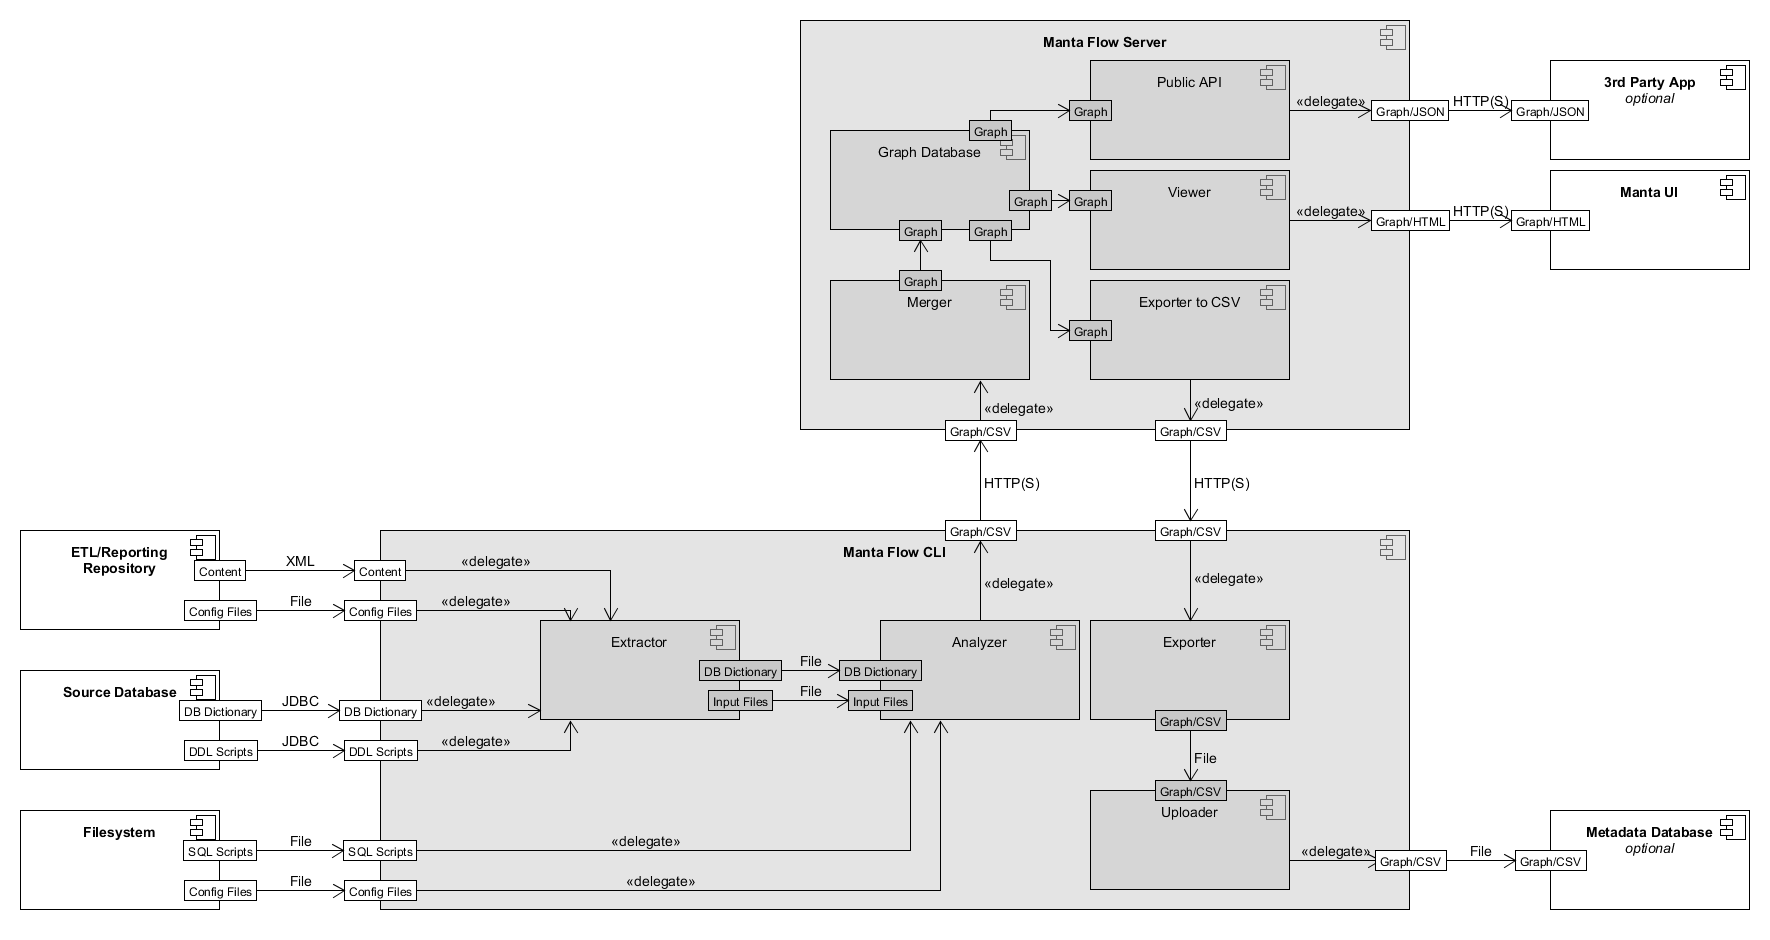
\includegraphics[width=14cm]{figures/flow_comp}
\caption{Architektura \textit{Manta Flow}}
\label{fig:ana-flow-comp}
\end{center}
\end{figure}

\begin{figure}
\begin{center}
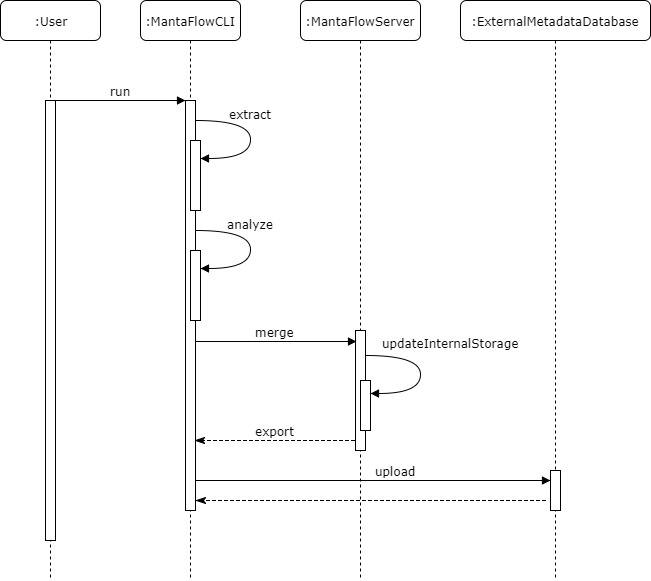
\includegraphics[width=14cm]{figures/flow_seq}
\caption{Interakce mezi \textit{klientskou} a \textit{serverovou} částí \textit{Manta Flow}}
\label{fig:ana-flow-seq}
\end{center}
\end{figure}

\subsection{Metadatové uložiště}
\label{sec:ana_model}
Jak již bylo zmíněno v úvodu práce (kapitola \ref{sec:uvod}) metadatové uložiště produktu \textit{Manta Flow} je aktuálně implementováno grafovou databází \textit{Titan} (ve verzi 0.4) a je snaha o výměnu této databáze\cite{Kovar18}. 
Než přistoupíme k bližšímu popisu jednotlivých komponent aplikace a jejich interakcí s metadatovým uložištěm (kapitola \ref{sec:ana_components}, je třeba nejdříve popsat entity, které jsou součástí analýzy datových toků a datový model metadatového uložiště (zobrazený na obrázku \ref{fig:ana-model}\footnote{Z modelu metadatového uložiště je zřejmé, že ne všechny podgrafy tvoří \textit{strom}. Vlastnosti \textit{stromu} nicméně porušují pouze hrany typu \textit{directFlow} a \textit{filterFlow}, které jsou výsledkem analýzy datových toků a jejichž odstraněním by strom vznikl. V textu je tak v některých případech používána teminologie vztahující se ke \textit{stromům} (například \textit{kořen}) - na celý graf je nahlíženo jako ne \textit{les}.}). 

% entity datového modelu
V procesu analýzy datových toků hraje roli mnoho entit z analyzovaných systémů. Ty se navíc mohou výrazně lišit systém od systému - \textit{Manta Flow} může analyzovat širokou škálu spolu propojených databázových systémů a integračních služeb. Obecně lze říci, že každý systém obsahuje zdroje a cíle dat (tabulky, soubory, ...) a transformace dat (skripty, \textit{\nomExpl{ETL}{Extract Load Transform}} workflow, procedury, makra a další).

\begin{figure}
\begin{center}
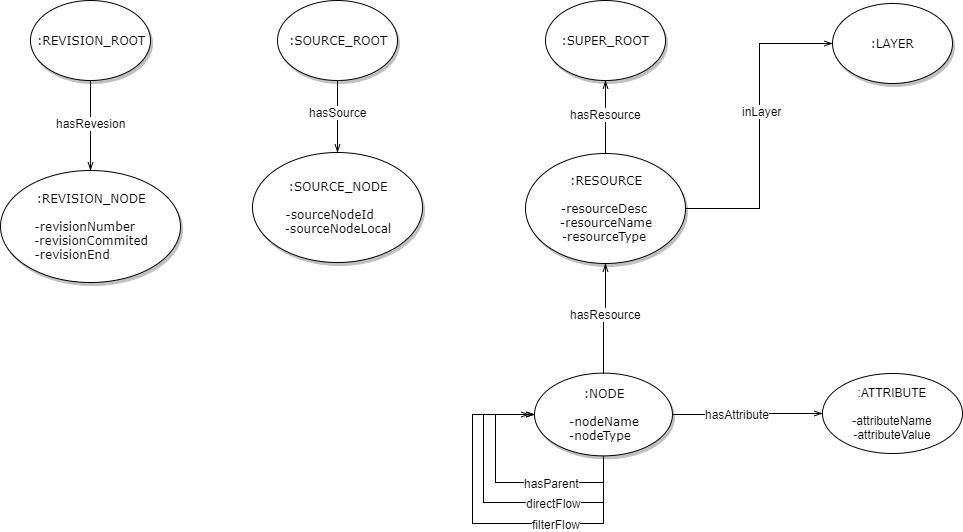
\includegraphics[width=14cm]{figures/model}
\caption{Model grafové databáze}
\label{fig:ana-model}
\end{center}
\end{figure}

% datový model
Samotný datový model se skládá z devíti typů uzlů:

\begin{itemize}
	\item{\textit{SUPER\_ROOT}}: Uzel (právě jeden v databázi), který slouží jako umělý kořen všech uzlů typu \textit{RESOURCE}. 
	\item{\textit{RESOURCE}}: Uzly tohoto typu reprezentují zdrojové systémy - zdroje definic objektů, zdrojových kódů, ETL řešení a další.  
	\item{\textit{NODE}}: Uzly typu \textit{NODE} představují reálné objekty zdrojového systému - databáze, tabulky, sloupce, procedury, skripty a další. 
	\item{\textit{LAYER}}: Uzly typu \textit{LAYER} reprezentují vrstvy modelu metadat. Datové toky nalezené při analýze zdrojových kódů jsou vždy ukládány do \textit{fyzické vrstvy}, ze které je potom možné generovat abstraktnější vrstvy modelu datových toků.  
	\item{\textit{ATTRIBUTE}}: Uzly typu \textit{ATTRIBUTE} reprezentují atributy uzlů typu \textit{NODE} - parametry sloupců, popisy databázových objektů a další.
	\item{\textit{SOURCE\_ROOT}}: Uzel (právě jeden v databázi), který slouží jako umělý kořen všech uzlů typu \textit{SOURCE\_NODE}. 
	\item{\textit{SOURCE\_NODE}}: Uzly typu \textit{SOURCE\_NODE} reprezentují soubory se zdrojovými kódy extrahovanými ze zdrojových systémů. 
	\item{\textit{REVISION\_ROOT}}: Uzel (právě jeden v databázi), který slouží jako umělý kořen všech uzlů typu \textit{REVISION\_NODE}. 
	\item{\textit{REVISION\_NODE}}: Uzly typu \textit{ATTRIBUTE} reprezentují revize modelu metadat, definují tedy jeho verzování. Kromě dalších parametrů mají všechny hrany grafu parametry \textit{tranEnd} a \textit{tranStart} definující platnost hran (viz obrázek \ref{fig:ana-model-rev}). Při každé analýze zdrojových systémů (která je prováděna dávkově klientskou částí aplikace) je vytvořena nová revize metadatového uložiště obsahující všechny objekty zdrojových systémů.\footnote{Je snaha tento princip upravit tak, aby byly objekty v metadatovém uložišti minimálně repklikovány \cite{Sykora17}.}  
\end{itemize}

 a osmi typů hran:

 \begin{itemize}
	\item{\textit{hasResource}}: Hrana přiřazuje objekty (uzly typu \textit{NODE}) ke svým zdrojovým systémům (uzlům typu \textit{RESOURCE}). Hrana je také použite k propojení uzlů typu \textit{RESOURCE} s uzlem \textit{RESOURCE\_ROOT}.
	\item{\textit{hasParent}}: Hrana mezi dvěmi uzly typu \textit{NODE} vytvářející klasickou hiearchickou strukturu mezi těmito uzly - strom závislostí objektů zdrojových systémů. 
	\item{\textit{directFlow}}: Hrana mezi dvěmi uzly typu \textit{NODE} říkající, že mezi těmito uzly existuje přímý datový tok (ve směru hrany).
	\item{\textit{filterFlow}}: Hrana mezi dvěmi uzly typu \textit{NODE} říkající, že mezi těmito uzly existuje nepřímý datový tok (ve směru hrany).
	\item{\textit{hasAttribute}}: Hrana přiřazující uzlům typu \textit{NODE} jejich atributy (uzly typu \textit{ATTRIBUTE}).
	\item{\textit{inLayer}}: Hrana typu \textit{inLayer} spojeju zdroje (uzly typu \textit{RESOURCE}) a vrstvy a říká, že zdroj patří do dané vrstvy modelu metadat. 
	\item{\textit{hasSource}}: Hrana je použita k propojení uzlů reprezentujících zdrojové kódy (uzly typu \textit{SOURCE\_NODE}) s uzlem \textit{SOURCE\_ROOT}.
	\item{\textit{hasRevision}}: Hrana je použita k propojení uzlů reprezentujících revize modelu metadat (uzly typu \textit{REVISION\_NODE}) s uzlem \textit{REVISION\_ROOT}.
\end{itemize}

\begin{figure}
\begin{center}
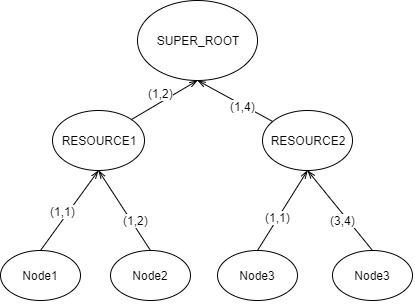
\includegraphics[width=6cm]{figures/model_revisions}
\caption{Způsob verzování modelu metadat}
\label{fig:ana-model-rev}
\end{center}
\end{figure}

Uzly i hrany mají dle svého typu několik specifických atributů, ty ale nebudeme blíže popisovat, protože nejsou pro analýzu zásadní. 

V metadatovém uložišti je dále definováno několik typů indexů, konkrétně se jedná o standardní indexy:

\begin{itemize}
	\item{\textit{indexy na kořeny}}: indexy pro konkrétní uzly, kořeny jednotlivých stromů datového modelu - \textit{SUPER\_ROOT, SOURCE\_ROOT, REVISION\_ROOT}
	\item{\textit{indexy na atributy hran}}: indexy zrychlující dohledávání atributů hran
	\item{\textit{indexy na typy hran}}: indexy zrychlující dohledávání hran daného typu pro jednotlivé uzly
\end{itemize}

a externí \textit{Apache Lucene} indexy, které slouží pro \textit{fulltextové} vyhledávání uzlů dle jejich názvů a pro intervalové vyhledání revizí. 

\subsection{Popis komponent}
\label{sec:ana_components}

Aplikace \textit{Manta Flow} praceje s metadatovým uložištěm několika různými způsoby, přičemž různé moduly aplikace využívají jeden či více těchto přístupů (a často také provádí vlastní pomocné dotazy přímo do metadatového uložiště). Cílem této sekce je tyto způsoby manipulace s metadatovým uložištěm identifikovat a popsat (není tedy účelem detailní technický popis všech dotazů do metadatového uložiště, ale spíše popis obecných principů a specifických situací - například netradiční zacházení s transakcemi). 

\subsubsection{Connector}
\label{sec:ana_connector}
Modul, který je nejblíže metadatovému uložišti, tzv. \textbf{connector} má dvě hlavní zodpovědnosti - zajištění připojení aplikace k uložišti a provádění dotazů nad ním. 

%Operations
Modul obsahuje sadu základních dotazů, tzv. \textit{operatinos}, mezi které patří například: 
\begin{itemize}
	\item{získání předka uzlu}
	\item{získání atributů uzlu}
	\item{získání sousedních uzlů a hran}
	\item{získání cesty ke kořeni}
	\item{získání podstromu}
\end{itemize} 
Tyto operace přímo přistupují do databáze a pomocí programovacího jazyka \textit{Gremlin}\footnote{Používá se \textit{TinkerPop} ve verzi \textit{2.6}.} a jsou na nich postaveny složitější operace nad grafouvou databází. U základních operací nejsou transakce řízeny explicitně, ale implicitně grafovou databází.

% Algorithm
Další částí modulu \textit{connector} jsou tzv. algoritmy, tedy komponenta, pomocí které jsou v metadatovém uložišti hledány samotné datové toky. Tato komponenta řetězí několik grafových algoritmů, přičemž první z nich získá z metadatového uložiště podmnožinu datových toků, která je dalšími algoritmy filtrována a omezována. Tímto způsobem vzniká tzv. \textit{referenční view} - objekt obsahující kompletní graf datových toků pro zadané výchozí uzly a směr datových toků. To je pak využ   íváno dalšími moduly aplikace, například \textit{viewerem} (viz \ref{sec:ana_viewer}), který dle parametrů zadaných ve webové aplikaci graf datových toků vizualizuje.
Jednotlivé algoritmy používají výše popsané základní operace (\textit{operations}) a v některých případech také samy dotazují metadatové uložiště přímo pomocí jazyka \textit{Gremlin}. 

% Traversal
Posledním způsobem manipulace s metadatovým uložištěm, který modul umožňuje je přístup pomocí \textit{traverserů}. Ty pracují na obecném principu \textit{traversování} grafů popsaném v kapitole \ref{sec:gdb-dotazy}. V tomto případě ale celý průchod grafem není realizován samotnou grafovou databází, ale přímo aplikací, přičemž grafová databáze je dotazována pouze na dílčí informace - například na okolní uzly. \textit{Traversery} jsou používány v případech, kdy je manipulováno s větší částí grafové databáze, například při jejím exportu. Tyto operace jsou realizovány \textit{vizitory} - každý uzel, který je procházen \textit{traverserem} je následně obsloužen \textit{vizitorem}, který provede požadovanou operaci (jedná se o návrhový vzor \textit{Visitor} - viz \cite{Gamma94}). Obě tyto části, tedy procházení grafu \textit{traverserem} i obsloužení všech objektů \textit{visitorem} jsou prováděny za pomocí základních grafových operací definovaných výše (\textit{operations}). Zároveň je ale také z tohoto kontextu grafová databáze dotazována přímo pomocí jazyka \textit{Gremlin}. Jedná se ale spíše o jednoduché dotazy na dohledání uzlů, jejich atributů apod. 

\subsubsection{Query}
Modul \textit{query} do jisté míry rozšiřuje modul \textit{connector}. Obsahuje pomocné funkce pro hledání datových toků (resp. \textit{referenčního view}), konfiguraci algoritmů poskytovaných \textit{connectorem} a sadu jednoduchých dotazů do metadatového uložiště. 

\subsubsection{Merger}
\textit{Merger} je modul, který je používán při analýze zdrojových systémů. Slouží k zanesení výsledků dílčích analýz jednotlivých částí (např. skriptů) zdrojových systémů do metadatového uložiště. 

Vlastní operace \textit{merge}\footnote{Operace \textit{merge} má v kontextu aplikace \textit{Manta Flow} obdobný význam, jako například v \textit{SQL}: pokud objekt není uložen v persistentní vrstvě, je do ní uložen (\textit{insert}), jinak je aktualizován (\textit{update}).} lze zjednodušeně popsat pseudokódem \ref{alg_merger}. Ten je uveden především kvůli složitému mode zanořování transakcí, jehož účelem je umožňení provádění dotazů do metadatového uložiště jinými částmi aplikace, zatímco je prováděn \textit{merge} analyzoných částí zdrojových systémů. % TODO blíže popsat použitý transakční model

Operace se chová různě v případě, kdy je umožňěno verzovaní metadatového uložiště (a to tak obsahuje více revízí) a kdy je vypnuto. V případě zapnutého verzování je \textit{merge} prováděn vždy do nové revize, pokud je verzování vypnuté, je prováděn do hlavní (jediné) revize. 

Samotné \textit{merge} operace nad objekty grafové databáze (uzly, hranami, atributy, ...) jsou prováděny přímímy dotazy do databáze pomocí jazyka \textit{Gremlin}. K přístupu do metadadtového uložiště se tedy nevyužívá modul k tomu předurčený - \textit{Connector} (viz \ref{sec:ana_connector}).

\begin{algorithm} 
\caption{Merger pseudocode}
\label{alg_merger}
\begin{algorithmic}
	\State $beginWriteTransaction()$
	\State $revision\gets getNewestRevision()$
	\If {$revision.isOpen()$}
		\State $beginWriteTransaction()$
		\ForAll{$script in scripts$} 
			\State $beginWriteTransaction()$
			\State $merge(script)$	
			\State $conditionalCommit()$
		\EndFor
		\State $beginWriteTransaction()$
		\ForAll{$object in objects$} 
			\State $beginWriteTransaction()$
			\State $merge(object)$	
			\State $occasionalCommit()$
		\EndFor
		\State $commit()$	
	\EndIf
	\State $commit()$
\end{algorithmic}
\end{algorithm}

\subsubsection{Viewer}
\label{sec:ana_viewer}
\textit{Viewer} je modul sloužící k poskytování dat uživatelskému rozhraní aplikace (klientské části webové aplikace). Jeho nejčastější interakce s metadatovým uložištěm je dotaz na \textit{referenční view} dle parametrů zadaných uživatelem. To je prováděno pomocí algoritmů definovaných v modulu \textit{connector} (viz \ref{sec:ana_connector}) a modulu \textit{query}, který obsahuje pomocné funkce pro hledání datových toků (resp. \textit{referenčního view}) a konfiguraci algoritmů poskytovaných \textit{connectorem}.

Kromě toho \textit{viewer} dotazuje metadatové uložiště o další informace, které následně propaguje do uživatelského rozhraní - především o informace o revizích metadatového uložiště a o objekty zdrojových systémů, pomocí kterých uživatel vybírá výchozí uzly pro hledání datových toků (\textit{referenčního view}). Informace o revizích metadatového uložiště jsou dohledávány pomocí základních operací definovaných v modulu \textit{connector} (viz \ref{sec:ana_connector}) a pomocí přímých dotazů do metadatového uložiště pomocí jazyka \textit{Gremlin} s explicitního řízení transakcí. Pro vyhledávání objektů zdrojových systémů (v metadatovém uložišti uzly typu \textit{NODE}, viz \ref{sec:ana_model}) je použito vyhledávání pomocí fulltextového indexu implementovaného pomocí \textit{Apache Lucene}. Ten indexuje uzly v metadatovém uložišti podle jejich názvu a umožňuje jejich rychlé vyhledávání. 


\subsubsection{Public API}
\label{sec:ana_public}
\textit{Public API} je modul, který by měl umožňovat vzdálené volání veřejné části funkcionality aplikace pomocí \textit{REST API}. Konkrétně lze tímto způsobem volat například analýzu datových toků mezi různými objekty zdrojového systému. Modul přepoužívá část funkcionality poskytovanou moduly \textit{connector} a \textit{query}, část těchto funkcionalit ale duplikuje (s menšími úpravami) a přímo tak dotazuje metadatové uložiště.    

\subsubsection{Exporter}
\label{sec:ana_exporter}
Posledním modulem, který přímo interaguje s metadatovým uložištěm je \textit{exporter}, jehož úkolem je exportovat aktuální stav grafové databáze (ne nutně vše, může být exportován například jen interval revizí atd.) buďto do \textit{CSV} souborů, nebo přímo do formátu používaného dalšími nástroji používanými na správu metadat. \textit{Exporter} jako nástroj pro práci s metadatovým uložištěm nejčastěji používá \textit{traversery} a \textit{observery} poskytované modulem \textit{connector}, díky kterým je možné provádět operace nad velkou částí metadatového uložiště bez zásadních paměťových požadavků. Dále jsou využívány základní základní operace (\textit{operations}) poskytované stejným modulem a v některých případech je metadatové uložiště dotazováno přímo pomocí jazyka \textit{Gremlin}.

%todo možná závěr podsekce s diagramem závislostí modulů

% TODO POPIS API jednotlivých databází
\subsection{API grafových databází}
\label{sec:ana_gdbapi}
\textit{Manta Flow} pro dotazování grafové databáze (v tuto chvíli \textit{Titan}) používá programovací jazyk \textit{Gremlin} ve verzi \textit{2.6}. Lze tedy říci, že tento programovací jazyk slouží jako API mezi aplikací a aktuálně používanou grafovou databází. Z benchmarků dalších grafových databází \cite{Kovar18} vyplývá, že bude-li současná grafová databáze nahrazena, jejím nástupcem bude pravděpodobně \textit{JanusGraph}, nebo \textit{OrientDB}\textit{Všechny zmíněné databáze jsou blíže popsány v kapitole \ref{sec:gdb-databaze}.}. %TODO obě tyto db používají gremlin (asi)

%TODO
\subsection{Požadavky}
%security 
% - podle rolí
% - nevidím flow v cizích systémech, ale vidím, že z vlastního tam flow vede

% - Není nutné upravovat algoritmus pro hledání flow  				--- stačí najít kompletní flow se všmi objekty a odfiltrovat zakázané.
% - Úprava algoritmu pro hledání flow by alg. nezrychlila 			--- stejně by bylo nutné hledat přes zakázané objekty (pro případ, že za nimi jsou ještě viditelné objekty, které jsou součástí flow)
% ==> Neupravovat algoritmy, natož DB dotazy
% ==> Nalezená flow by měla být filtrována -> sw. vrstva - na jaké úrovni? 
% - Filtrovat by se mělo až ve chvíli, kdy je flow kompletní 
% - - 






% Podněty
% - Architektura vyhovující cloudovým požadavkům
%  - žádný filesystem, jen pipes na jiné služby, které mohou filesystem podporovat (lze využívat pouze temp uložiště a sfree buckety)
%  - např jedna služba client, jedna server, jedna grafovka
%  - jak by se řešily veškeré konfigurace



%%%%%%%%%%%%%%%%%%%%%%%%%% 
% Seznam literatury je v samostatnem souboru reference.bib. 
\bibliographystyle{csplainnat}
{
\def\CS{$\cal C\kern-0.1667em\lower.5ex\hbox{$\cal S$}\kern-0.075em $}
\bibliography{reference}
}

%%%%%%%%%%%%%%%%%%%%%%%%%% 
% vše co následuje bude uvedeno v přílohách
\appendix	

\printnomenclature
\label{apx:zkratky}

\chapter{Obsah přiloženého CD}

TODO

\end{document}
